\documentclass[dvipdfmx]{jsarticle}
\setcounter{section}{6}
\setcounter{subsection}{4}
\usepackage{xr}
\externaldocument{4.5.4}
\externaldocument{4.6.1}
\externaldocument{4.6.2}
\externaldocument{4.6.3}
\usepackage{amsmath,amsfonts,amssymb,array,comment,mathtools,url,docmute}
\usepackage{longtable,booktabs,dcolumn,tabularx,mathtools,multirow,colortbl,xcolor}
\usepackage[dvipdfmx]{graphics}
\usepackage{bmpsize}
\usepackage{amsthm}
\usepackage{enumitem}
\setlistdepth{20}
\renewlist{itemize}{itemize}{20}
\setlist[itemize]{label=•}
\renewlist{enumerate}{enumerate}{20}
\setlist[enumerate]{label=\arabic*.}
\setcounter{MaxMatrixCols}{20}
\setcounter{tocdepth}{3}
\newcommand{\rotin}{\text{\rotatebox[origin=c]{90}{$\in $}}}
\newcommand{\amap}[6]{\text{\raisebox{-0.7cm}{\begin{tikzpicture} 
  \node (a) at (0, 1) {$\textstyle{#2}$};
  \node (b) at (#6, 1) {$\textstyle{#3}$};
  \node (c) at (0, 0) {$\textstyle{#4}$};
  \node (d) at (#6, 0) {$\textstyle{#5}$};
  \node (x) at (0, 0.5) {$\rotin $};
  \node (x) at (#6, 0.5) {$\rotin $};
  \draw[->] (a) to node[xshift=0pt, yshift=7pt] {$\textstyle{\scriptstyle{#1}}$} (b);
  \draw[|->] (c) to node[xshift=0pt, yshift=7pt] {$\textstyle{\scriptstyle{#1}}$} (d);
\end{tikzpicture}}}}
\newcommand{\twomaps}[9]{\text{\raisebox{-0.7cm}{\begin{tikzpicture} 
  \node (a) at (0, 1) {$\textstyle{#3}$};
  \node (b) at (#9, 1) {$\textstyle{#4}$};
  \node (c) at (#9+#9, 1) {$\textstyle{#5}$};
  \node (d) at (0, 0) {$\textstyle{#6}$};
  \node (e) at (#9, 0) {$\textstyle{#7}$};
  \node (f) at (#9+#9, 0) {$\textstyle{#8}$};
  \node (x) at (0, 0.5) {$\rotin $};
  \node (x) at (#9, 0.5) {$\rotin $};
  \node (x) at (#9+#9, 0.5) {$\rotin $};
  \draw[->] (a) to node[xshift=0pt, yshift=7pt] {$\textstyle{\scriptstyle{#1}}$} (b);
  \draw[|->] (d) to node[xshift=0pt, yshift=7pt] {$\textstyle{\scriptstyle{#2}}$} (e);
  \draw[->] (b) to node[xshift=0pt, yshift=7pt] {$\textstyle{\scriptstyle{#1}}$} (c);
  \draw[|->] (e) to node[xshift=0pt, yshift=7pt] {$\textstyle{\scriptstyle{#2}}$} (f);
\end{tikzpicture}}}}
\renewcommand{\thesection}{第\arabic{section}部}
\renewcommand{\thesubsection}{\arabic{section}.\arabic{subsection}}
\renewcommand{\thesubsubsection}{\arabic{section}.\arabic{subsection}.\arabic{subsubsection}}
\everymath{\displaystyle}
\allowdisplaybreaks[4]
\usepackage{vtable}
\theoremstyle{definition}
\newtheorem{thm}{定理}[subsection]
\newtheorem*{thm*}{定理}
\newtheorem{dfn}{定義}[subsection]
\newtheorem*{dfn*}{定義}
\newtheorem{axs}[dfn]{公理}
\newtheorem*{axs*}{公理}
\renewcommand{\headfont}{\bfseries}
\makeatletter
  \renewcommand{\section}{%
    \@startsection{section}{1}{\z@}%
    {\Cvs}{\Cvs}%
    {\normalfont\huge\headfont\raggedright}}
\makeatother
\makeatletter
  \renewcommand{\subsection}{%
    \@startsection{subsection}{2}{\z@}%
    {0.5\Cvs}{0.5\Cvs}%
    {\normalfont\LARGE\headfont\raggedright}}
\makeatother
\makeatletter
  \renewcommand{\subsubsection}{%
    \@startsection{subsubsection}{3}{\z@}%
    {0.4\Cvs}{0.4\Cvs}%
    {\normalfont\Large\headfont\raggedright}}
\makeatother
\makeatletter
\renewenvironment{proof}[1][\proofname]{\par
  \pushQED{\qed}%
  \normalfont \topsep6\p@\@plus6\p@\relax
  \trivlist
  \item\relax
  {
  #1\@addpunct{.}}\hspace\labelsep\ignorespaces
}{%
  \popQED\endtrivlist\@endpefalse
}
\makeatother
\renewcommand{\proofname}{\textbf{証明}}
\usepackage{tikz,graphics}
\usepackage[dvipdfmx]{hyperref}
\usepackage{pxjahyper}
\hypersetup{
 setpagesize=false,
 bookmarks=true,
 bookmarksdepth=tocdepth,
 bookmarksnumbered=true,
 colorlinks=false,
 pdftitle={},
 pdfsubject={},
 pdfauthor={},
 pdfkeywords={}}
\begin{document}
%\hypertarget{riemannux7a4dux5206}{%
\subsection{Riemann積分}%\label{riemannux7a4dux5206}}
%\hypertarget{ux533aux9593ux584aux4e0aux306eriemannux7a4dux5206}{%
\subsubsection{区間塊上のRiemann積分}%\label{ux533aux9593ux584aux4e0aux306eriemannux7a4dux5206}}\par
Lebesgue積分について述べる前にLebesgue測度の基本的なことについて述べておこう。
\begin{dfn*}[定義\ref{区間}の再掲]
$n$次元数空間$\mathbb{R}^{n}$において、$\forall i \in \varLambda_{n}$に対し、$- \infty \leq a_{i} \leq b_{i} \leq \infty$なる元々$a_{i}$、$b_{i}$を用いて次式のように書かれる集合$I$を$n$次元の区間ということにする。定義から分かるように、空集合もまた$n$次元の区間である。このような区間全体の集合を以下$\mathfrak{I}_{n}$と書くことにする。
\begin{align*}
I = \left\{ \mathbf{x} \in \mathbb{R}^{n} \middle| \mathbf{x} = \left( x_{i} \right)_{i \in \varLambda_{n}},\ \ \forall i \in \varLambda_{n}\left[ a_{i} < x_{i} \leq b_{i} \right] \right\} = \prod_{i \in \varLambda_{n}} \left( a_{i},b_{i} \right]
\end{align*}
\end{dfn*}
\begin{dfn*}[定義\ref{区間塊}の再掲]
その集合$\mathfrak{I}_{n}$の互いに素な元の族$\left\{ I_{i} \right\}_{i \in \varLambda_{m} }$が与えられたとき、これの直和$\bigsqcup_{i \in \varLambda_{m} } I_{i}$を$n$次元の区間塊ということにする。定義から明らかに空集合もまた$n$次元の区間である。このような区間塊全体の集合を以下$\mathfrak{F}_{n}$と書くことにする。
\end{dfn*}
\begin{dfn*}[定義\ref{有限加法的なLebesgue-Stieltjes測度}の再掲]
$\forall i \in \varLambda_{n}$に対し、関数$f_{i}:\mathbb{R} \rightarrow \mathbb{R}$が単調増加するようなその関数$F = \left( f_{i} \right)_{i \in \varLambda_{n}}:\mathbb{R} \rightarrow \mathbb{R}^{n}$が与えられたとき、次式のように写像$\psi_{F}:\mathfrak{I}_{n} \rightarrow \mathrm{cl}\mathbb{R}^{+}$が定義される。また、$\psi_{F}(\emptyset) = 0$と定義される。
\begin{align*}
\psi_{F}(I) = \sup\left\{ \prod_{i \in \varLambda_{n}} \left( f_{i}\left( b_{i}' \right) - f_{i}\left( a_{i}' \right) \right) \in \mathrm{cl}\mathbb{R}^{+} \middle| \forall\prod_{i \in \varLambda_{n}} \left( a_{i}',b_{i}' \right]\in \mathfrak{P}(I) \cap \mathfrak{I}_{n} \right\}
\end{align*}
さらに、次式のようにgraphが$G_{\varPsi_{F}}$の対応$\varPsi_{F}:\mathfrak{F}_{n} \multimap \mathrm{cl}\mathbb{R}^{+}$が定義される。
\begin{align*}
G_{\varPsi_{F}} = \left\{ (E,S) \in \mathfrak{F}_{n} \times \mathrm{cl}\mathbb{R}^{+} \middle| S = \sum_{i \in \varLambda_{m}} {\psi_{F}\left( I_{i} \right)},\ \ E = \bigsqcup_{i \in \varLambda_{m}} I_{i},\ \ \left\{ I_{i} \right\}_{i \in \varLambda_{m}} \subseteq \mathfrak{I}_{n} \right\}
\end{align*}
このような対応$\varPsi_{F}$は、実はのちに述べるように、写像どころかJordan測度をも成していることから、そのJordan測度$\varPsi_{F}:\mathfrak{F}_{n} \rightarrow \mathrm{cl}\mathbb{R}^{+}$を、ここでは、その関数$F:\mathbb{R} \rightarrow \mathbb{R}^{n}$についての有限加法的なLebesgue-Stieltjes測度ということにする。
\end{dfn*}
\begin{dfn*}[定義\ref{Lebesgue-Stieltjes測度}の再掲]
$F = \left( f_{i} \right)_{i \in \varLambda_{n}}$なる関数$F:\mathbb{R} \rightarrow \mathbb{R}^{n}$について、$i \in \varLambda_{n}$なる単調増加する関数たち$f_{i}:\mathbb{R} \rightarrow \mathbb{R}$が右連続であるときのその有限加法的なLebesgue-Stieltjes測度$\varPsi_{F}$を関数$F:\mathbb{R} \rightarrow \mathbb{R}^{n}$についてのLebesgue-Stieltjes測度という。
\end{dfn*}
\begin{dfn*}[定義\ref{Lebesgue測度}の再掲]
集合$\mathbb{R}$の恒等写像$I_{\mathbb{R}}$は明らかに右連続であるから、$\forall i \in \varLambda_{n}$に対し、$f_{i} = I_{\mathbb{R}}$のときの有限加法的なLebesgue-Stieltjes測度、Lebesgue-Stieltjes外測度、Lebesgue-Stieltjes測度、Lebesgue-Stieltjes可測集合の全体の集合をそれぞれ有限加法的なLebesgue測度、Lebesgue外測度、Lebesgue測度、Lebesgue可測集合の全体の集合といい、それぞれ、$l:\mathfrak{F}_{n} \rightarrow \mathrm{cl}\mathbb{R}^{+}$、$\lambda^{*}\mathfrak{:P}\left( \mathbb{R}^{n} \right) \rightarrow \mathrm{cl}\mathbb{R}^{+}$、$\lambda:\mathfrak{M}_{C}\left( \lambda^{*} \right) \rightarrow \mathrm{cl}\mathbb{R}^{+}$、$\mathfrak{M}_{C}\left( \lambda^{*} \right)$と書くことにする。
\end{dfn*}\par
以下ここでは、関数$F = \left( I_{\mathbb{R}} \right)_{i \in \varLambda_{n}}:\mathbb{R} \rightarrow \mathbb{R}^{n}$についての写像$\psi_{F}:\mathfrak{I}_{n} \rightarrow \mathrm{cl}\mathbb{R}^{+}$が$\psi$とおかれることにする。
\begin{thm}\label{4.6.5.1}
上で定義された写像$\psi:\mathfrak{I}_{n} \rightarrow \mathrm{cl}\mathbb{R}^{+}$について、$I = \prod_{i \in \varLambda_{n}} \left( a_{i},b_{i} \right]$なる区間$I$が有界な区間であるとき、次式が成り立つ。
\begin{align*}
\psi(I) = \prod_{i \in \varLambda_{n}} \left( b_{i} - a_{i} \right)
\end{align*}
\end{thm}
\begin{proof} 定理\ref{4.5.4.1}より明らかである。
\end{proof}
\begin{thm}\label{4.6.5.2}
$n$次元の区間全体の集合$\mathfrak{I}_{n}$に制限されたその対応$l|\mathfrak{I}_{n}$は上の写像$\psi$に等しくなる。
\end{thm}
\begin{proof}
その集合$\mathfrak{I}_{n}$に制限されたその対応$l|\mathfrak{I}_{n}$において、$\forall I \in \mathfrak{I}_{n}$に対し、元の族$\left\{ I \right\}$もやはりその集合$\mathfrak{I}_{n}$の元の族でもあるから、次式が成り立つ。
\begin{align*}
l|\mathfrak{I}_{n}(I) = l(I) = \varPsi(I)
\end{align*}
\end{proof}
\begin{thm}\label{4.6.5.3}
$\forall E \in \mathfrak{F}_{n}$に対し、次式が成り立つかつ、互いに素なその集合$\mathfrak{I}_{n}$の元の族$\left\{ I_{i} \right\}_{i \in \varLambda_{m}}$が与えられたとき、
\begin{align*}
E = \bigsqcup_{i \in \varLambda_{m}} I_{i}
\end{align*}
上で定義された対応$l$によるその集合$E$の値はその族$\left\{ I_{i} \right\}_{i \in \varLambda_{m}}$によらなくその対応$l$は写像になる。
\end{thm}
\begin{proof} 定理\ref{4.5.4.3}より明らかである。
\end{proof}
\begin{thm}\label{4.6.5.4}
先ほどの写像$l:\mathfrak{F}_{n} \rightarrow \mathrm{cl}\left( \mathbb{R}^{+} \right)$はJordan測度である。さらに、これはその集合$\mathfrak{F}_{n}$上で完全加法的である。
\end{thm}
\begin{proof} 定理\ref{4.5.4.4}、定理\ref{4.5.4.5}より明らかである。
\end{proof}
\begin{thm}\label{4.6.5.5}
$l = \lambda^{*}|\mathfrak{F}_{n}$が成り立ち、このとき、その有限加法的なLebesgue測度$l$はLebesgue可測集合の全体の集合$\mathfrak{M}_{C}\left( \lambda^{*} \right)$で定義された測度であり測度空間を次式のように与える。
\begin{align*}
\left( \mathbb{R}^{n},\mathfrak{M}_{C}\left( \lambda^{*} \right),\lambda^{*} \right) = \left( \mathbb{R}^{n},\varSigma_{l}^{\star},l^{\star} \right)
\end{align*}
\end{thm}
\begin{proof} 定理\ref{4.6.5.4}より有限加法的なLebesgue測度$l$は完全加法的である。このとき、定理\ref{4.5.3.2}より$l = \lambda^{*}|\mathfrak{F}_{n}$が成り立つ。また、定理\ref{4.5.3.13}よりその有限加法的なLebesgue測度$l$はLebesgue可測集合の全体の集合$\mathfrak{M}_{C}\left( \lambda^{*} \right)$で定義された測度であり測度空間を次式のように与える。
\begin{align*}
\left( \mathbb{R}^{n},\mathfrak{M}_{C}\left( \lambda^{*} \right),\lambda^{*}|\mathfrak{M}_{C}\left( \lambda^{*} \right) \right) = \left( \mathbb{R}^{n},\varSigma_{l}^{\star},l^{\star} \right)
\end{align*}
\end{proof}
\begin{dfn}
$\forall E \in \mathfrak{F}_{n}$に対し、$E = \bigsqcup_{i \in \varLambda_{N}} I_{i}$なるその集合$\mathfrak{I}_{n}$の族$\left\{ I_{i} \right\}_{i \in \varLambda_{N} }$が与えられる。これをその区間塊$E$の分割といい、これ全体の集合を$\mathcal{D}(E)$と書く。さらに、$\xi_{i} \in I_{i}$なる点$\xi_{i}$をその区間$I_{i}$の代表点という。
\end{dfn}
\begin{dfn}
$\forall E \in \mathfrak{F}_{n}\forall\varDelta \in \mathcal{D}(E)$に対し、$\varDelta = \left\{ I_{i} \right\}_{i \in \varLambda_{N} }$と与えられたとき、実数$\max_{i \in \varLambda_{N}}{\sup_{\mathbf{a},\mathbf{b} \in I_{i}}\left\| \mathbf{b} - \mathbf{a} \right\|}$をその分割$\varDelta$の幅といいこれを$\mathcal{M}(\varDelta)$と書くことにする。
\end{dfn}
\begin{dfn}
$\forall E \in \mathfrak{F}_{m}\forall\varDelta \in \mathcal{D}(E)$に対し、関数$f:E \rightarrow \mathbb{R}^{n}$が与えられ、さらに、$\varDelta = \left\{ I_{i} \right\}_{i \in \varLambda_{N}}$と与えられたとき、$\xi_{i} \in I_{i}$なる代表点の族$\left\{ \xi_{i} \right\}_{i \in \varLambda_{N}}$がとられてこれが$\Xi$とおかれて作られた次式のような和$S_{R}(f,\varDelta,\Xi)$をその関数$f$のその分割$\varDelta$とその族$\Xi$によるRiemann和という。なお、$\lambda$は$n$次元数空間$\mathbb{R}^{n}$でのLebesgue測度である。
\begin{align*}
S_{R}(f,\varDelta,\Xi) = \sum_{i \in \varLambda_{N}} {f\left( \xi_{i} \right)\lambda\left( I_{i} \right)}
\end{align*}
\end{dfn}
\begin{dfn}
$\forall E \in \mathfrak{F}_{m}\forall\varDelta \in \mathcal{D}(E)$に対し、関数$f:E \rightarrow \mathbb{R}^{n}$を用いて、あるvectors$\mathbf{I}$が存在して、分割$\varDelta$をなす区間の代表点の族$\Xi$によらず次式が成り立つとき、
\begin{align*}
\mathbf{I} = \lim_{\scriptsize \begin{matrix}
\mathcal{M}(\varDelta) \rightarrow 0 \\
\varDelta \in \mathcal{D}(E) \\
\end{matrix}}{S_{R}(f,\varDelta,\Xi)}
\end{align*}
その関数$f$はその区間塊$E$でRiemann積分可能であるといい、さらに、vectors$\mathbf{I}$をその関数$f$のその区間塊$E$上のRiemann積分といい次のように書く。
\begin{align*}
\mathbf{I} = \int_{E} f = \int_{E} {f\left( \mathbf{x} \right)d\mathbf{x}}
\end{align*}
\end{dfn}
\begin{thm}\label{4.6.5.6}
$\forall E \in \mathfrak{F}_{m}\forall\varDelta \in \mathcal{D}(E)$に対し、関数$f:E \rightarrow \mathbb{R}^{n}$がその区間塊$E$でRiemann積分可能であるとき、そのRiemann積分はただ1つである。
\end{thm}
\begin{proof}
$\forall E \in \mathfrak{F}_{m}\forall\varDelta \in \mathcal{D}(E)$に対し、関数$f:E \rightarrow \mathbb{R}^{n}$がその区間塊$E$でRiemann積分可能であるとき、そのRiemann積分が$\mathbf{I}$、$\mathbf{J}$と与えられたなら、次式が成り立つ。
\begin{align*}
\mathbf{I} = \lim_{\scriptsize \begin{matrix}
\mathcal{M}(\varDelta) \rightarrow 0 \\
\varDelta \in \mathcal{D}(E) \\
\end{matrix}}{S_{R}(f,\varDelta,\Xi)},\ \ \mathbf{J} = \lim_{\scriptsize \begin{matrix}
\mathcal{M}(\varDelta) \rightarrow 0 \\
\varDelta \in \mathcal{D}(E) \\
\end{matrix}}{S_{R}(f,\varDelta,\Xi)}
\end{align*}
このとき、$\forall\varepsilon \in \mathbb{R}^{+}\exists\delta_{\mathbf{I}},\delta_{\mathbf{J}} \in \mathbb{R}^{+}$に対し、$\mathcal{M}(\varDelta) < \delta_{\mathbf{I}}$が成り立つなら、$\left\| S_{R}(f,\varDelta,\Xi) - \mathbf{I} \right\| < \varepsilon$が成り立つかつ、$\mathcal{M}(\varDelta) < \delta_{\mathbf{J}}$が成り立つなら、$\left\| S_{R}(f,\varDelta,\Xi) - \mathbf{J} \right\| < \varepsilon$が成り立つ。そこで、$\delta = \min\left\{ \delta_{\mathbf{I}},\delta_{\mathbf{J}} \right\}$とおかれれば、$\mathcal{M}(\varDelta) < \delta_{\mathbf{I}}$が成り立つなら、$\left\| S_{R}(f,\varDelta,\Xi) - \mathbf{I} \right\| < \varepsilon$が成り立つかつ、$\left\| S_{R}(f,\varDelta,\Xi) - \mathbf{J} \right\| < \varepsilon$が成り立つので、次のようになる。
\begin{align*}
0 &\leq \left\| \mathbf{I} - \mathbf{J} \right\|\\
&= \left\| \mathbf{I} - S_{R}(f,\varDelta,\Xi) + S_{R}(f,\varDelta,\Xi) - \mathbf{J} \right\|\\
&\leq \left\| \mathbf{I} - S_{R}(f,\varDelta,\Xi) \right\| + \left\| S_{R}(f,\varDelta,\Xi) - \mathbf{J} \right\|\\
&= \left\| S_{R}(f,\varDelta,\Xi) - \mathbf{I} \right\| + \left\| S_{R}(f,\varDelta,\Xi) - \mathbf{J} \right\| < 2\varepsilon
\end{align*}
したがって、$\left\| \mathbf{I} - \mathbf{J} \right\| = 0$、即ち、$\mathbf{I} = \mathbf{J}$が成り立つ。
\end{proof}
\begin{thm}\label{4.6.5.7}
$\forall E \in \mathfrak{F}_{m}$に対し、関数$f:E \rightarrow \mathbb{R}^{n}$がその区間塊$E$でRiemann積分可能であるならそのときに限り、$f = \left( f_{k} \right)_{k \in \varLambda_{n}}$とおかれれば、その関数$f_{k}$もRiemann積分可能であり次式が成り立つ\footnote{特に、$\mathbb{R}^{n} = \mathbb{C}$のとき、$f = g + ih$とおかれれば、次式が成り立つ。
\begin{align*}
\int_{E} f = \int_{E} g + i\int_{E} h
\end{align*}}。
\begin{align*}
\int_{E} f = \left( \int_{E} f_{k} \right)_{k \in \varLambda_{n}}
\end{align*}
\end{thm}
\begin{proof}
$\forall E \in \mathfrak{F}_{m}$に対し、関数$f:E \rightarrow \mathbb{R}^{n}$がその区間塊$E$でRiemann積分可能であるとき、定義より、$\forall\varDelta \in \mathcal{D}(E)$に対し、$f = \left( f_{k} \right)_{k \in \varLambda_{n}}$、$\varDelta = \left\{ I_{i} \right\}_{i \in \varLambda_{N}}$、$\Xi = \left\{ \xi_{i} \right\}_{i \in \varLambda_{N}}$とおかれれば、分割$\varDelta$をなす区間の代表点の族$\Xi$によらず次のようになることから、
\begin{align*}
\int_{E} f &= \lim_{\scriptsize \begin{matrix}
\mathcal{M}(\varDelta) \rightarrow 0 \\
\varDelta \in \mathcal{D}(E) \\
\end{matrix}}{S_{R}(f,\varDelta,\Xi)}\\
&= \lim_{\scriptsize \begin{matrix}
\mathcal{M}(\varDelta) \rightarrow 0 \\
\varDelta \in \mathcal{D}(E) \\
\end{matrix}}{\sum_{i \in \varLambda_{N}} {f\left( \xi_{i} \right)\lambda\left( I_{i} \right)}}\\
&= \lim_{\scriptsize \begin{matrix}
\mathcal{M}(\varDelta) \rightarrow 0 \\
\varDelta \in \mathcal{D}(E) \\
\end{matrix}}{\sum_{i \in \varLambda_{N}} {\left( f_{k} \right)_{k \in \varLambda_{n}}\left( \xi_{i} \right)\lambda\left( I_{i} \right)}}\\
&= \lim_{\scriptsize \begin{matrix}
\mathcal{M}(\varDelta) \rightarrow 0 \\
\varDelta \in \mathcal{D}(E) \\
\end{matrix}}\left( \sum_{i \in \varLambda_{N}} {f_{k}\left( \xi_{i} \right)\lambda\left( I_{i} \right)} \right)_{k \in \varLambda_{n}}\\
&= \left( \lim_{\scriptsize \begin{matrix}
\mathcal{M}(\varDelta) \rightarrow 0 \\
\varDelta \in \mathcal{D}(E) \\
\end{matrix}}{\sum_{i \in \varLambda_{N}} {f_{k}\left( \xi_{i} \right)\lambda\left( I_{i} \right)}} \right)_{k \in \varLambda_{n}}\\
&= \left( \lim_{\scriptsize \begin{matrix}
\mathcal{M}(\varDelta) \rightarrow 0 \\
\varDelta \in \mathcal{D}(E) \\
\end{matrix}}{S_{R}\left( f_{k},\varDelta,\Xi \right)} \right)_{k \in \varLambda_{n}}\\
&= \left( \int_{E} f_{k} \right)_{k \in \varLambda_{n}}
\end{align*}
その関数$f_{k}$はその区間塊$E$でRiemann積分可能である。逆も同様にして示される。
\end{proof}
%\hypertarget{ux4e0bux7a4dux5206ux3068ux4e0aux7a4dux5206}{%
\subsubsection{下積分と上積分}%\label{ux4e0bux7a4dux5206ux3068ux4e0aux7a4dux5206}}
\begin{dfn}
$\forall E \in \mathfrak{F}_{m}\forall\varDelta \in \mathcal{D}(E)$に対し、関数$f:E \rightarrow \mathbb{R}$が与えられ、さらに、$\varDelta = \left\{ I_{i} \right\}_{i \in \varLambda_{N}}$と与えられたとき、次式のような和々$s(f,\varDelta)$、$S(f,\varDelta)$をそれぞれその関数$f$のその分割$\varDelta$による不足和、過剰和という。なお、$\lambda$は$m$次元数空間$\mathbb{R}^{m}$でのLebesgue測度である。
\begin{align*}
s(f,\varDelta) = \sum_{i \in \varLambda_{N}} {\inf{f|I_{i}}\lambda\left( I_{i} \right)},\ \ S(f,\varDelta) = \sum_{i \in \varLambda_{N}} {\sup{f|I_{i}}\lambda\left( I_{i} \right)}
\end{align*}
\end{dfn}
\begin{dfn}
$\forall E \in \mathfrak{F}_{m}$に対し、関数$f:E \rightarrow \mathbb{R}^{n}$を用いて、$f = \left( f_{k} \right)_{k \in \varLambda_{n}}$とおかれれば、あるvectors$\mathbf{I}$、$\mathbf{J}$が存在して、次式が成り立つとき、
\begin{align*}
\mathbf{I} = \left( \sup_{\varDelta \in \mathcal{D}(E)}{s\left( f_{k},\varDelta \right)} \right)_{k \in \varLambda_{n}},\ \ \mathbf{J} = \left( \inf_{\varDelta \in \mathcal{D}(E)}{S\left( f_{k},\varDelta \right)} \right)_{k \in \varLambda_{n}}
\end{align*}
その関数$f$はそれぞれその区間塊$E$で下積分可能である、上積分可能であるといい、さらに、それらの実数たち$\mathbf{I}$、$\mathbf{J}$をその関数$f$のその区間塊$E$上の下積分、上積分といい次のように書く。
\begin{align*}
\mathbf{I} = s_{E}f = s_{E}f\left( \mathbf{x} \right)d\mathbf{x},\ \ \mathbf{J} = S_{E}f = S_{E}f\left( \mathbf{x} \right)d\mathbf{x}
\end{align*}
\end{dfn}
\begin{thm}\label{4.6.5.8}
$\forall E \in \mathfrak{F}_{m}$に対し、関数$f:E \rightarrow \mathbb{R}^{n}$がその区間塊$E$で下積分可能である、上積分可能であるとき、$f = \left( f_{k} \right)_{k \in \varLambda_{n}}$とおかれれば、次式が成り立つ\footnote{特に、$\mathbb{R}^{n} = \mathbb{C}$のとき、$f = g + ih$とおかれれば、次式が成り立つ。
\begin{align*}
s_{E}f = s_{E}g + is_{E}h,\ \ S_{E}f = S_{E}g + iS_{E}h
\end{align*}}。
\begin{align*}
s_{E}f = \left( s_{E}f_{k} \right)_{k \in \varLambda_{n}},\ \ S_{E}f = \left( S_{E}f_{k} \right)_{k \in \varLambda_{n}}
\end{align*}
\end{thm}
\begin{proof} 定義より明らかである。
\end{proof}
%\hypertarget{ux7d30ux5206}{%
\subsubsection{細分}%\label{ux7d30ux5206}}
\begin{dfn}
$\forall E \in \mathfrak{F}_{n}$に対し、有界な関数$f:E \rightarrow \mathbb{R}$が与えられたとき、実数$\sup f - \inf f$をその関数$f$のその区間塊$E$における振幅という。
\end{dfn}
\begin{thm}\label{4.6.5.9}
$\forall E \in \mathfrak{F}_{n}$に対し、有界な関数$f:E \rightarrow \mathbb{R}$が与えられたとき、次式が成り立つ。
\begin{align*}
\sup_{\mathbf{x},\mathbf{y} \in E}\left| f\left( \mathbf{x} \right) - f\left( \mathbf{y} \right) \right| = \sup f - \inf f
\end{align*}
\end{thm}
\begin{proof}
$\forall E \in \mathfrak{F}_{n}$に対し、有界な関数$f:E \rightarrow \mathbb{R}$が与えられたとき、$\forall\mathbf{x},\mathbf{y} \in E$に対し、$\inf f \leq f\left( \mathbf{x} \right) \leq \sup f$かつ$\inf f \leq f\left( \mathbf{y} \right) \leq \sup f$が成り立つので、次のようになる。
\begin{align*}
\left\{ \begin{matrix}
\inf f \leq f\left( \mathbf{x} \right) \leq \sup f \\
\inf f \leq f\left( \mathbf{y} \right) \leq \sup f \\
\end{matrix} \right. &\Leftrightarrow \left\{ \begin{matrix}
\inf f \leq f\left( \mathbf{x} \right) \leq \sup f \\
 - \sup f \leq - f\left( \mathbf{y} \right) \leq - \inf f \\
\end{matrix} \right.\ \\
&\Rightarrow \inf f - \sup f \leq f\left( \mathbf{x} \right) - f\left( \mathbf{y} \right) \leq \sup f - \inf f\\
&\Leftrightarrow \left| f\left( \mathbf{x} \right) - f\left( \mathbf{y} \right) \right| \leq \sup f - \inf f
\end{align*}
このとき、$\exists\varepsilon \in \mathbb{R}^{+}\forall\mathbf{x} \in E$に対し、$\varepsilon \leq \sup f - f\left( \mathbf{x} \right)$が成り立つと仮定すると、$f\left( \mathbf{x} \right) \leq \sup f - \varepsilon$が成り立ち、次式のようにおかれれば、
\begin{align*}
U\left( V(f) \right) = \left\{ a \in \mathbb{R} \middle| \forall\mathbf{x} \in E\left[ f\left( \mathbf{x} \right) \leq a \right] \right\}
\end{align*}
その関数$f$は有界なので、$\sup f = \min{U\left( V(f) \right)}$が成り立つのであった。一方で、$\forall\mathbf{x} \in E$に対し、$f\left( \mathbf{x} \right) < \sup f - \varepsilon$が成り立つので、$\sup f - \varepsilon \in U\left( V(f) \right)$が得られる。したがって、$\sup f = \min{U\left( V(f) \right)} \leq \sup f - \varepsilon$が得られ$\varepsilon \leq 0$が成り立つ。しかしながら、これは$0 < \varepsilon$が成り立つことに矛盾している。ゆえに、$\forall\varepsilon \in \mathbb{R}^{+}\exists\mathbf{x} \in E$に対し、$0 \leq \sup f - f\left( \mathbf{x} \right) < \varepsilon$が成り立つ。同様にして、$\forall\varepsilon \in \mathbb{R}^{+}\exists\mathbf{y} \in E$に対し、$0 \leq f\left( \mathbf{y} \right) - \inf f < \varepsilon$が成り立つ。したがって、上記の議論により次のようになる。
\begin{align*}
\left\{ \begin{matrix}
0 \leq \sup f - f\left( \mathbf{x} \right) < \varepsilon \\
0 \leq f\left( \mathbf{y} \right) - \inf f < \varepsilon \\
\end{matrix} \right. &\Rightarrow 0 \leq \left( \sup f - \inf f \right) - \left( f\left( \mathbf{x} \right) - f\left( \mathbf{y} \right) \right) < 2\varepsilon\\
&\Rightarrow 0 \leq \left| f\left( \mathbf{x} \right) - f\left( \mathbf{y} \right) \right| \leq \sup f - \inf f < 2\varepsilon + \left( f\left( \mathbf{x} \right) - f\left( \mathbf{y} \right) \right) = \left| 2\varepsilon + \left( f\left( \mathbf{x} \right) - f\left( \mathbf{y} \right) \right) \right| \leq 2\varepsilon + \left| f\left( \mathbf{x} \right) - f\left( \mathbf{y} \right) \right|\\
&\Rightarrow \sup_{\mathbf{x},\mathbf{y} \in E}\left| f\left( \mathbf{x} \right) - f\left( \mathbf{y} \right) \right| \leq \sup f - \inf f < \sup_{\mathbf{x},\mathbf{y} \in E}\left| f\left( \mathbf{x} \right) - f\left( \mathbf{y} \right) \right| + 2\varepsilon\\
&\Leftrightarrow 0 \leq \sup f - \inf f - \sup_{\mathbf{x},\mathbf{y} \in E}\left| f\left( \mathbf{x} \right) - f\left( \mathbf{y} \right) \right| < 2\varepsilon
\end{align*}
したがって、次式が成り立つ。
\begin{align*}
\sup_{\mathbf{x},\mathbf{y} \in E}\left| f\left( \mathbf{x} \right) - f\left( \mathbf{y} \right) \right| = \sup f - \inf f
\end{align*}
\end{proof}
\begin{dfn}
$\forall E \in \mathfrak{F}_{n}$に対し、これの2つの分割たち$\varGamma$、$\varDelta$がそれぞれ$\left\{ I_{i} \right\}_{i \in \varLambda_{M}}$、$\left\{ J_{j} \right\}_{j \in \varLambda_{N}}$と与えられたとき、$\forall j \in M$に対し、あるその集合$\varLambda_{M}$の部分集合$\varLambda_{j}$が存在して、$J_{j} = \bigsqcup_{i \in \varLambda_{j}} I_{i}$が成り立つとき、その分割$\varGamma$はその分割$\varDelta$の細分といい$\varGamma \preccurlyeq \varDelta$と書くことにする。
\end{dfn}
\begin{thm}\label{4.6.5.10}
$\forall E \in \mathfrak{F}_{n}$に対し、組$\left( \mathcal{D}(E), \preccurlyeq \right)$は順序集合をなす、即ち、次のことが成り立つ。
\begin{itemize}
\item
  $\forall\varDelta \in \mathcal{D}(E)$に対し、$\varDelta \preccurlyeq \varDelta$が成り立つ。
\item
  $\forall\varGamma,\varDelta \in \mathcal{D}(E)$に対し、$\varGamma \preccurlyeq \varDelta$かつ$\varDelta \preccurlyeq \varGamma$が成り立つなら、$\varGamma = \varDelta$が成り立つ。
\item
  $\forall B,\varGamma,\varDelta \in \mathcal{D}(E)$に対し、$B \preccurlyeq \varGamma$かつ$\varGamma \preccurlyeq \varDelta$が成り立つなら、$B \preccurlyeq \varDelta$が成り立つ。
\end{itemize}
\end{thm}
\begin{proof}
$\forall E \in \mathfrak{F}_{n}$に対し、組$\left( \mathcal{D}(E), \preccurlyeq \right)$について、$\forall\varDelta \in \mathcal{D}(E)$に対し、この分割$\varDelta$が$\left\{ I_{i} \right\}_{i \in \varLambda_{N}}$と与えられたらば、$\forall i \in \varLambda$に対し、$I_{i} = \bigsqcup_{i' \in \left\{ i \right\}} I_{i'}$が成り立つので、もちろん、$\varDelta \preccurlyeq \varDelta$が成り立つ。\par
$\forall\varGamma,\varDelta \in \mathcal{D}(E)$に対し、$\varGamma \preccurlyeq \varDelta$かつ$\varDelta \preccurlyeq \varGamma$が成り立つなら、これらの分割たち$\varGamma$、$\varDelta$がそれぞれ$\left\{ I_{i} \right\}_{i \in \varLambda_{M}}$、$\left\{ J_{j} \right\}_{j \in \varLambda_{N}}$とおかれれば、$\forall j \in \varLambda_{N}$に対し、あるその集合$\varLambda_{M}$の部分集合$\varLambda_{j}$が存在して、$J_{j} = \bigsqcup_{i \in \varLambda_{j}} I_{i}$が成り立つかつ、$\forall i \in \varLambda_{M}$に対し、あるその集合$\varLambda_{N}$の部分集合$\varLambda_{i}$が存在して、$I_{i} = \bigsqcup_{j \in \varLambda_{i}} J_{j}$が成り立つので、$\forall j \in \varLambda_{N}$に対し、次のことが成り立つ。
\begin{align*}
J_{j} = \bigsqcup_{i \in \varLambda_{j}} I_{i} = \bigsqcup_{i \in \varLambda_{j}} {\bigsqcup_{j' \in \varLambda_{i}} J_{j'}} = \bigsqcup_{\forall i \in \varLambda_{j}\left[ j' \in \varLambda_{i} \right]} J_{j'}
\end{align*}
そこで、区間塊の定義よりその添数$j'$のとり方が1通りしかないので、その添数$j'$の添数集合が$\varLambda'$とおかれれば、次のことが成り立つ。
\begin{align*}
1 = \#\left\{ j \right\} \leq \#\varLambda_{j} \leq \#\varLambda' = 1
\end{align*}
これにより、$\#\varLambda_{j} = 1$が成り立つので、$\varLambda_{j} = \left\{ i \right\}$とおかれれば、$\forall j \in \varLambda_{N}$に対し、あるその集合$\varLambda$の添数$i$がただ1つ存在して、$J_{j} = I_{i}$が成り立つ。これにより、$\varGamma = \varDelta$が成り立つ。\par
$\forall B,\varGamma,\varDelta \in \mathcal{D}(E)$に対し、$B \preccurlyeq \varGamma$かつ$\varGamma \preccurlyeq \varDelta$が成り立つなら、これらの分割たち$B$、$\varGamma$、$\varDelta$がそれぞれ$\left\{ I_{i} \right\}_{i \in \varLambda_{L} }$、$\left\{ J_{j} \right\}_{j \in \varLambda_{M} }$、$\left\{ K_{k} \right\}_{k \in \varLambda_{N} }$とおかれれば、$\forall j \in \varLambda_{M}$に対し、あるその集合$\varLambda_{L}$の部分集合$\varLambda_{j}$が存在して、$J_{j} = \bigsqcup_{i \in \varLambda_{j}} I_{i}$が成り立つかつ、$\forall k \in \varLambda_{N}$に対し、あるその集合$\varLambda_{M}$の部分集合$\varLambda_{k}$が存在して、$K_{k} = \bigsqcup_{j \in \varLambda_{k}} J_{j}$が成り立つので、以上の議論により、次のようになる。
\begin{align*}
K_{k} = \bigsqcup_{j \in \varLambda_{k}} J_{j} = \bigsqcup_{j \in \varLambda_{k}} {\bigsqcup_{i \in \varLambda_{j}} I_{i}} = \bigsqcup_{\forall j \in \varLambda_{k}\left[ i \in \varLambda_{j} \right]} I_{i}
\end{align*}
これにより、$B \preccurlyeq \varDelta$が成り立つ。
\end{proof}
\begin{thm}\label{4.6.5.11}
$\forall E \in \mathfrak{F}_{n}\forall\varGamma,\varDelta \in \mathcal{D}(E)$に対し、有界な関数たち$f:E \rightarrow \mathbb{R}$、$g:E \rightarrow \mathbb{R}$が与えられたとき、次のことが成り立つ。なお、$\lambda$は$n$次元数空間$\mathbb{R}^{n}$でのLebesgue測度である。
\begin{itemize}
\item
  $\inf f\lambda(E) \leq s(f,\varDelta) \leq S(f,\varDelta) \leq \sup f\lambda(E)$が成り立つ。
\item
  $\varGamma \preccurlyeq \varDelta$が成り立つなら、$s(f,\varDelta) \leq s(f,\varGamma) \leq S(f,\varGamma) \leq S(f,\varDelta)$が成り立つ。
\item
  $s(f,\varGamma) \leq S(f,\varDelta)$が成り立つ。
\item
  $s_{E}f \leq S_{E}f$が成り立つ。
\item
  $f \leq g$が成り立つなら、$s_{E}f \leq s_{E}g$かつ$S_{E}f \leq S_{E}g$が成り立つ。
\end{itemize}
\end{thm}
\begin{proof}
$\forall E \in \mathfrak{F}_{n}\forall\varDelta \in \mathcal{D}(E)$に対し、有界な関数たち$f:E \rightarrow \mathbb{R}$、$g:E \rightarrow \mathbb{R}$が与えられたとき、この分割$\varDelta$が$\left\{ I_{i} \right\}_{i \in \varLambda_{N}}$とおかれれば、$\inf f \leq \inf{f|I_{i}} \leq \sup{f|I_{i}} \leq \sup f$が成り立つ。これにより、次のようになる。なお、$\lambda$は$n$次元数空間$\mathbb{R}^{n}$でのLebesgue測度である。
\begin{align*}
\inf f\lambda(E) &= \inf f\lambda\left( \bigsqcup_{i \in \varLambda_{N}} I_{i} \right)\\
&= \inf f\sum_{i \in \varLambda_{N}} {\lambda\left( I_{i} \right)}\\
&= \sum_{i \in \varLambda_{N}} {\inf f\lambda\left( I_{i} \right)}\\
&\leq \sum_{i \in \varLambda_{N}} {\inf{f|I_{i}}\lambda\left( I_{i} \right)} = s(f,\varDelta)\\
&\leq \sum_{i \in \varLambda_{N}} {\sup{f|I_{i}}\lambda\left( I_{i} \right)} = S(f,\varDelta)\\
&\leq \sum_{i \in \varLambda_{N}} {\sup f\lambda\left( I_{i} \right)}\\
&= \sup f\sum_{i \in \varLambda_{N}} {\lambda\left( I_{i} \right)}\\
&= \sup f\lambda\left( \bigsqcup_{i \in \varLambda_{N}} I_{i} \right)\\
&= \sup f\lambda(E)
\end{align*}\par
$\forall\varGamma,\varDelta \in \mathcal{D}(E)$に対し、$\varGamma \preccurlyeq \varDelta$が成り立つなら、これらの分割たち$\varGamma$、$\varDelta$がそれぞれ$\left\{ I_{i} \right\}_{i \in \varLambda_{M}}$、$\left\{ J_{j} \right\}_{j \in \varLambda_{N}}$とおかれれば、$\forall j \in \varLambda_{N}$に対し、あるその集合$\varLambda_{M}$の部分集合$\varLambda_{j}$が存在して、$J_{j} = \bigsqcup_{i \in \varLambda_{j}} I_{i}$が成り立つ。これにより、$\forall i \in \varLambda_{j}$に対し、$\inf{f|J_{j}} \leq \inf{f|I_{i}}$かつ$\sup{f|I_{i}} \leq \sup{f|J_{j}}$が成り立つので、次のようになる。
\begin{align*}
s(f,\varDelta) &= \sum_{j \in \varLambda_{N}} {\inf{f|J_{j}}\lambda\left( J_{j} \right)}\\
&= \sum_{j \in \varLambda_{N}} {\inf{f|J_{j}}\lambda\left( \bigsqcup_{i \in \varLambda_{j}} I_{i} \right)}\\
&= \sum_{j \in \varLambda_{N}} {\inf{f|J_{j}}\sum_{i \in \varLambda_{j}} {\lambda\left( I_{i} \right)}}\\
&= \sum_{j \in \varLambda_{N}} {\sum_{i \in \varLambda_{j}} {\inf{f|J_{j}}\lambda\left( I_{i} \right)}}\\
&\leq \sum_{j \in \varLambda_{N}} {\sum_{i \in \varLambda_{j}} {\inf{f|I_{i}}\lambda\left( I_{i} \right)}}\\
&= \sum_{i \in \varLambda_{M}} {\inf{f|I_{i}}\lambda\left( I_{i} \right)} = s(f,\varGamma)
\end{align*}
同様にして、$S(f,\varGamma) \leq S(f,\varDelta)$が成り立つことも示される。あとは上記の議論により$s(f,\varGamma) \leq S(f,\varGamma)$も成り立つ。\par
$\forall\varGamma,\varDelta \in \mathcal{D}(E)$に対し、これらの分割たち$\varGamma$、$\varDelta$がそれぞれ$\left\{ I_{i} \right\}_{i \in \varLambda_{M}}$、$\left\{ J_{j} \right\}_{j \in \varLambda_{N}}$とおかれれば、$\forall(i,j),(k,l) \in \varLambda_{M} \times \varLambda_{N}$に対し、$(i,j) \neq (k,l)$が成り立つなら、$i \neq k$または$j \neq l$が成り立つので、$i \neq k$のとき、次のようになる。
\begin{align*}
\left( I_{i} \cap J_{j} \right) \cap \left( I_{k} \cap J_{l} \right) &= \left( I_{i} \cap I_{k} \right) \cap J_{j} \cap J_{l}\\
&= \emptyset \cap J_{j} \cap J_{l} = \emptyset
\end{align*}
$j \neq l$のときも同様にして、$\left( I_{i} \cap J_{j} \right) \cap \left( I_{k} \cap J_{l} \right) = \emptyset$が成り立つことが示される。また、次のようになるので、
\begin{align*}
\bigsqcup_{(i,j) \in \varLambda_{M} \times \varLambda_{N}} \left( I_{i} \cap J_{j} \right) &= \bigcup_{i \in \varLambda_{M}} {\bigcup_{j \in \varLambda_{N}} \left( I_{i} \cap J_{j} \right)}\\
&= \bigcup_{i \in \varLambda_{M}} \left( I_{i} \cap \bigcup_{j \in \varLambda_{N}} J_{j} \right)\\
&= \bigcup_{i \in \varLambda_{M}} \left( I_{i} \cap E \right) = \bigcup_{i \in \varLambda_{M}} I_{i} = E
\end{align*}
その族$\left\{ I_{i} \cap J_{j} \right\}_{(i,j) \in \varLambda_{M} \times \varLambda_{N}}$もその区間塊$E$の分割でもある。さらに、$\forall i \in \varLambda_{M}$に対し、あるその集合$\varLambda_{M} \times \varLambda_{N}$の部分集合$\left( \varLambda_{M} \times \varLambda_{N} \right)_{i}$が存在して、$I_{i} = \bigsqcup_{\left( i',j' \right) \in \left( \varLambda_{M} \times \varLambda_{N} \right)_{i}} \left( I_{i'} \cap J_{j'} \right)$が成り立つかつ、$\forall j \in \varLambda_{N}$に対し、あるその集合$\varLambda_{M} \times \varLambda_{N}$の部分集合$\left( \varLambda_{M} \times \varLambda_{N} \right)_{j}$が存在して、$J_{j} = \bigsqcup_{\left( i',j' \right) \in \left( \varLambda_{M} \times \varLambda_{N} \right)_{j}} \left( I_{i'} \cap J_{j'} \right)$が成り立つので、その族$\left\{ I_{i} \cap J_{j} \right\}_{(i,j) \in \varLambda_{M} \times \varLambda_{N}}$が$B$とおかれれば、$B \preccurlyeq \varGamma$かつ$B \preccurlyeq \varDelta$が成り立つ。これにより、上記の議論から$s(f,\varGamma) \leq s(f,B) \leq S(f,B) \leq S(f,\varDelta)$が得られる。\par
$\forall\varGamma,\varDelta \in \mathcal{D}(E)$に対し、上記の議論により$s(f,\varGamma) \leq S(f,\varDelta)$が成り立つので、その実数$S(f,\varDelta)$はその集合$\left\{ s(f,\varGamma) \in \mathbb{R} \middle| \varGamma \in \mathcal{D}(E) \right\}$の1つの上界となっている。これにより、次のようになるので、
\begin{align*}
s_{E}f = \sup_{\varGamma \in \mathcal{D}(E)}{s(f,\varGamma)} = \sup\left\{ s(f,\varGamma) \in \mathbb{R} \middle| \varGamma \in \mathcal{D}(E) \right\} \leq S(f,\varDelta)
\end{align*}
また、その下積分$s_{E}f$はその集合$\left\{ S(f,\varDelta) \in \mathbb{R} \middle| \varDelta \in \mathcal{D}(E) \right\}$の1つの下界となっているので、次のようになる。
\begin{align*}
s_{E}f \leq \inf\left\{ S(f,\varDelta) \in \mathbb{R} \middle| \varDelta \in \mathcal{D}(E) \right\} = \inf_{\varDelta \in \mathcal{D}(E)}{S(f,\varDelta)} = S_{E}f
\end{align*}
よって、$s_{E}f \leq S_{E}f$が成り立つ。\par
$f \leq g$が成り立つなら、$\forall\varDelta \in \mathcal{D}(E)$に対し、この分割$\varDelta$が$\left\{ I_{i} \right\}_{i \in \varLambda_{N} }$とおかれれば、$\forall i \in \varLambda$に対し、$\inf{f|I_{i}} \leq \inf{g|I_{i}}$が成り立つので、次のようになる。
\begin{align*}
s_{E}f &= \sup_{\varDelta \in \mathcal{D}(E)}{s(f,\varDelta)}\\
&= \sup_{\varDelta \in \mathcal{D}(E)}{\sum_{i \in \varLambda_{N}} {\inf{f|I_{i}}\lambda\left( I_{i} \right)}}\\
&\leq \sup_{\varDelta \in \mathcal{D}(E)}{\sum_{i \in \varLambda_{N}} {\inf{g|I_{i}}\lambda\left( I_{i} \right)}}\\
&= \sup_{\varDelta \in \mathcal{D}(E)}{s(g,\varDelta)} = s_{E}g
\end{align*}
同様にして、$S_{E}f \leq S_{E}g$が成り立つことが示される。
\end{proof}
%\hypertarget{darbouxux306eux5b9aux7406}{%
\subsubsection{Darbouxの定理}%\label{darbouxux306eux5b9aux7406}}
\begin{thm}[Darbouxの定理]\label{4.6.5.12}
$\forall E \in \mathfrak{F}_{m}$に対し、有界な関数$f:E \rightarrow \mathbb{R}^{n}$が与えられたとき、次式が成り立つ。
\begin{align*}
\lim_{\scriptsize \begin{matrix}
\mathcal{M}(\varDelta) \rightarrow 0 \\
\varDelta \in \mathcal{D}(E) \\
\end{matrix}}{s(f,\varDelta)} = s_{E}f,\ \ \lim_{\scriptsize \begin{matrix}
\mathcal{M}(\varDelta) \rightarrow 0 \\
\varDelta \in \mathcal{D}(E) \\
\end{matrix}}{S(f,\varDelta)} = S_{E}f
\end{align*}
この定理をDarbouxの定理という。
\end{thm}
\begin{proof}
$\forall E \in \mathfrak{F}_{m}$に対し、その集合の分割の1つ$\varDelta'$に属する区間$I$が考えられよう。有界な関数$f|I:I \rightarrow \mathbb{R}$が与えられたとき、$s_{I}f|I = \sup_{\varGamma \in \mathcal{D}(I)}{s\left( f|I,\varDelta \right)}$が成り立つことから、$\exists\varepsilon \in \mathbb{R}^{+}\forall\varDelta \in \mathcal{D}(I)$に対し、$\varepsilon \leq s_{I}f|I - s\left( f|I,\varDelta \right)$が成り立つと仮定しよう。このとき、$s\left( f|I,\varDelta \right) \leq s_{I}f|I - \varepsilon$が成り立つことからしたがって、その実数$s_{I}f|I - \varepsilon$はその集合$\left\{ s\left( f|I,\varDelta \right) \in \mathbb{R} \middle| \varDelta \in \mathcal{D}(I) \right\}$の下界である。これにより、次のようになる。
\begin{align*}
s_{I}f|I = \sup_{\varDelta \in \mathcal{D}(I)}{s\left( f|I,\varDelta \right)} = \sup\left\{ s\left( f|I,\varDelta \right) \in \mathbb{R} \middle| \varDelta \in \mathcal{D}(I) \right\} \leq s_{I}f|I - \varepsilon
\end{align*}
したがって、$\varepsilon \leq 0$が得られるが、これは$0 < \varepsilon$が成り立つことに矛盾している。これにより、$\forall\varepsilon \in \mathbb{R}^{+}\exists\varGamma \in \mathcal{D}(I)$に対し、$s_{I}f|I - s\left( f|I,\varGamma \right) < \varepsilon$が成り立つ。そこで、定理\ref{4.6.5.11}より$s\left( f|I,\varGamma \right) \leq s_{I}f|I$が成り立つので、$0 \leq s_{I}f|I - s\left( f|I,\varGamma \right) < \varepsilon$が成り立つ。\par
そこで、$\forall\varDelta \in \mathcal{D}(I)$に対し、これらの分割たち$\varGamma$、$\varDelta$がそれぞれ$\left\{ I_{i} \right\}_{i \in \varLambda_{M}}$、$\left\{ J_{j} \right\}_{j \in \varLambda_{N}}$とおかれれば、定理\ref{4.6.5.11}の証明と同様にしてその族$\left\{ I_{i} \cap J_{j} \right\}_{(i,j) \in \varLambda_{M} \times \varLambda_{N}}$もその区間塊$E$の分割でもあり、その族$\left\{ I_{i} \cap J_{j} \right\}_{(i,j) \in \varLambda_{M} \times \varLambda_{N}}$が$B$とおかれれば、$B \preccurlyeq \varGamma$かつ$B \preccurlyeq \varDelta$が成り立つことが示される。定理\ref{4.6.5.11}より$s\left( f|I,\varGamma \right) \leq s\left( f|I,B \right)$かつ$s\left( f|I,\varDelta \right) \leq s\left( f|I,B \right)$が成り立つ。\par
ここで、$I_{i} = \prod_{k \in \varLambda_{m}} \left( a_{ik},b_{ik} \right]$、$J_{j} = \prod_{k \in \varLambda_{m}} \left( a_{jk}',b_{jk}' \right]$、$e = \min_{\begin{matrix}
i \in \varLambda \\
k \in \varLambda_{m} \\
\end{matrix}}\left( b_{ik} - a_{ik} \right)$とおかれれば、$\mathcal{M}(\varDelta) < e$が成り立つとすることで、$\forall i \in \varLambda\forall j \in M\forall k \in \varLambda_{m}$に対し、次のようになる。
\begin{align*}
b_{jk}' - a_{jk}' &\leq \max_{\begin{matrix}
j \in \varLambda_{N} \\
k \in \varLambda_{m} \\
\end{matrix}}\left( b_{jk}' - a_{jk}' \right)\\
&\leq \max_{j \in \varLambda_{N}}{\sup_{\mathbf{a},\mathbf{b} \in J_{j}}\left\| \mathbf{b} - \mathbf{a} \right\|} = \mathcal{M}(\varDelta)\\
&< e = \min_{\begin{matrix}
i \in \varLambda \\
k \in \varLambda_{m} \\
\end{matrix}}\left( b_{ik} - a_{ik} \right)\\
&\leq b_{ik} - a_{ik}
\end{align*}
これにより、その分割$\varDelta$に属する区間$J$の各辺のどの小区間もその分割$\varGamma$に属する区間$K$の各辺の境界を高々1つしか含まないことが分かる。そこで、$\forall j \in \varLambda_{N}$に対し、区間$J_{j}$の各辺の開核が含むその分割$\varGamma$に属する区間$K$の各辺の境界の個数が$n_{j}$とおかれれば、$0 \leq n_{j} \leq n$が成り立つことになる。このとき、$\inf{f|I} \leq \inf{f|J_{j}} \leq \inf{f|I_{i} \cap J_{j}} \leq \sup{f|I}$が成り立つので、次のようにおかれれば、
\begin{align*}
d_{j} = \sum_{i \in \varLambda_{M}} {\left( \inf{f|I_{i} \cap J_{j}} - \inf{f|J_{j}} \right)\lambda\left( I_{i} \cap J_{j} \right)}
\end{align*}
$n_{j} = 0$のとき、$d_{j} = 0$が成り立ち、$0 < n_{j}$のとき、次のようになる。
\begin{align*}
d_{j} &= \sum_{i \in \varLambda_{M}} {\left( \inf{f|I_{i} \cap J_{j}} - \inf{f|J_{j}} \right)\lambda\left( I_{i} \cap J_{j} \right)}\\
&\leq \sum_{i \in \varLambda_{M}} {\left( \sup{f|I} - \inf{f|I} \right)\lambda\left( I_{i} \cap J_{j} \right)}\\
&= \left( \sup{f|I} - \inf{f|I} \right)\sum_{i \in \varLambda_{M}} {\lambda\left( I_{i} \cap J_{j} \right)}\\
&= \left( \sup{f|I} - \inf{f|I} \right)\lambda\left( \bigsqcup_{i \in \varLambda_{M}} \left( I_{i} \cap J_{j} \right) \right)\\
&= \left( \sup{f|I} - \inf{f|I} \right)\lambda\left( \bigsqcup_{i \in \varLambda_{M}} I_{i} \cap J_{j} \right)\\
&= \left( \sup{f|I} - \inf{f|I} \right)\lambda\left( I \cap J_{j} \right)\\
&= \left( \sup{f|I} - \inf{f|I} \right)\lambda\left( J_{j} \right)
\end{align*}
これにより、次のようになる。
\begin{align*}
0 &\leq s\left( f|I,B \right) - s\left( f|I,\varDelta \right)\\
&= \sum_{(i,j) \in \varLambda \times M} {\inf{f|I_{i} \cap J_{j}}\lambda\left( I_{i} \cap J_{j} \right)} - \sum_{j \in \varLambda_{N}} {\inf{f|J_{j}}\lambda\left( J_{j} \right)}\\
&\leq \sum_{j \in \varLambda_{N}} {\sum_{i \in \varLambda_{M}} {\inf{f|I_{i} \cap J_{j}}\lambda\left( I_{i} \cap J_{j} \right)}} - \sum_{j \in \varLambda_{N}} {\inf{f|J_{j}}\lambda\left( I_{i} \cap J_{j} \right)}\\
&= \sum_{j \in \varLambda_{N}} \left( \sum_{i \in \varLambda_{M}} {\inf{f|I_{i} \cap J_{j}}\lambda\left( I_{i} \cap J_{j} \right)} - \inf{f|J_{j}}\lambda\left( I_{i} \cap J_{j} \right) \right)\\
&= \sum_{j \in \varLambda_{N}} \left( \sum_{i \in \varLambda_{M}} {\left( \inf{f|I_{i} \cap J_{j}} - \inf{f|J_{j}} \right)\lambda\left( I_{i} \cap J_{j} \right)} \right)\\
&= \sum_{j \in \varLambda_{N}} d_{j} = \sum_{\scriptsize \begin{matrix}
j \in \varLambda_{N} \\
n_{j} = 0 \\
\end{matrix}} d_{j} + \sum_{\scriptsize \begin{matrix}
j \in \varLambda_{N} \\
0 < n_{j} \\
\end{matrix}} d_{j} = \sum_{\scriptsize \begin{matrix}
j \in \varLambda_{N} \\
0 < n_{j} \\
\end{matrix}} d_{j}\\
&\leq \sum_{\scriptsize \begin{matrix}
j \in \varLambda_{N} \\
0 < n_{j} \\
\end{matrix}} {\left( \sup{f|I} - \inf{f|I} \right)\lambda\left( J_{j} \right)}\\
&= \left( \sup{f|I} - \inf{f|I} \right)\sum_{\scriptsize \begin{matrix}
j \in \varLambda_{N} \\
0 < n_{j} \\
\end{matrix}} {\lambda\left( J_{j} \right)}
\end{align*}\par
ここで、その区間$I$の辺$\left( a_{k},b_{k} \right]$の開核が含むその分割$\varGamma$に属する区間$J$の各辺の境界の個数が$r_{k}$とおかれれば、その分割$\varGamma$に属する区間$J$の各辺の境界をその区間$J_{j}$の各辺の開核が含むその区間$J_{j}$の和集合$\bigsqcup_{\scriptsize \begin{matrix}
j \in \varLambda_{N} \\
0 < n_{j} \\
\end{matrix} } J_{j}$について、次のようになる\footnote{いくらか不正確ではあるものの次の値々はそれぞれ横の図々の灰色部分の面積に該当する。なお、外枠が区間$I$で点線が分割$\varGamma$、実線が分割$\varDelta$である。\\
%\begin{comment}
\begin{tabular}{|C{\linewidth}{}{m}|C{0.5\linewidth}{}{m}|}
\hline
値 & 図 \nextRow
\hline \hline
$\lambda\left( \bigsqcup_{\scriptsize \begin{matrix}
  j \in \varLambda_{N} \\
  0 < n_{j} \\
\end{matrix}} J_{j} \right) $ & 
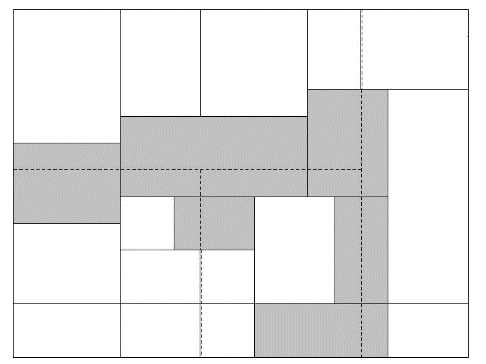
\includegraphics[width=54mm]{4.6.5.a.png} \nextRow
\hline
$\sum_{\scriptsize \begin{matrix}
  j \in \varLambda_{N} \\
  0 < n_{j} \\
\end{matrix}} {\max_{j \in \varLambda_{N}}{\sup_{\mathbf{a},\mathbf{b} \in J_{j}}\left\| \mathbf{b} - \mathbf{a} \right\|}\prod_{k' \in \varLambda_{m} \setminus \left\{ k \right\}} \left( b_{jk'} - a_{jk'} \right)}$ &
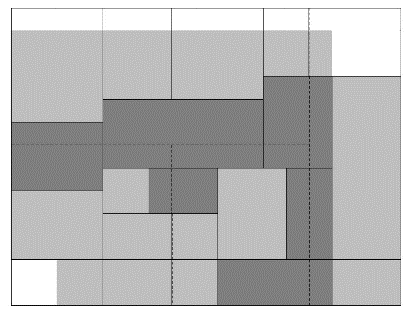
\includegraphics[width=54mm]{4.6.5.b.png} \nextRow
\hline
$\sum_{\scriptsize \begin{matrix}
  j \in \varLambda_{N} \\
  0 < n_{j} \\
\end{matrix}} {\max_{j \in \varLambda_{N}}{\sup_{\mathbf{a},\mathbf{b} \in J_{j}}\left\| \mathbf{b} - \mathbf{a} \right\|}\prod_{k' \in \varLambda_{m} \setminus \left\{ k \right\}} \left( b_{k'} - a_{k'} \right)}$ &
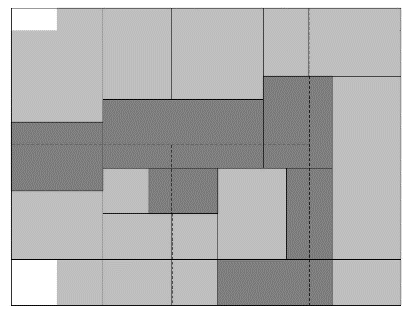
\includegraphics[width=54mm]{4.6.5.c.png} \nextRow
\hline
\end{tabular}}。
\begin{align*}
\lambda\left( \bigsqcup_{\scriptsize \begin{matrix}
j \in \varLambda_{N} \\
0 < n_{j} \\
\end{matrix} } J_{j} \right) &= \sum_{\scriptsize \begin{matrix}
j \in \varLambda_{N} \\
0 < n_{j} \\
\end{matrix}} {\lambda\left( J_{j} \right)} = \sum_{\scriptsize \begin{matrix}
j \in \varLambda_{N} \\
0 < n_{j} \\
\end{matrix}} {\prod_{k' \in \varLambda_{m}} \left( b_{jk'} - a_{jk'} \right)}\\
&= \sum_{\scriptsize \begin{matrix}
j \in \varLambda_{N} \\
0 < n_{j} \\
\end{matrix}} {\left( b_{jk'} - a_{jk'} \right)\prod_{k' \in \varLambda_{m} \setminus \left\{ k \right\}} \left( b_{jk'} - a_{jk'} \right)}\\
&\leq \sum_{\scriptsize \begin{matrix}
j \in \varLambda_{N} \\
0 < n_{j} \\
\end{matrix}} {\max_{j \in \varLambda_{N}}{\sup_{\mathbf{a},\mathbf{b} \in J_{j}}\left\| \mathbf{b} - \mathbf{a} \right\|}\prod_{k' \in \varLambda_{m} \setminus \left\{ k \right\}} \left( b_{jk'} - a_{jk'} \right)}\\
&\leq \sum_{\scriptsize \begin{matrix}
j \in \varLambda_{N} \\
0 < n_{j} \\
\end{matrix}} {\max_{j \in \varLambda_{N}}{\sup_{\mathbf{a},\mathbf{b} \in J_{j}}\left\| \mathbf{b} - \mathbf{a} \right\|}\prod_{k' \in \varLambda_{m} \setminus \left\{ k \right\}} \left( b_{k'} - a_{k'} \right)}\\
&= \sum_{k \in \varLambda_{m} } {r_{k}\max_{j \in \varLambda_{N}}{\sup_{\mathbf{a},\mathbf{b} \in J_{j}}\left\| \mathbf{b} - \mathbf{a} \right\|}\prod_{k' \in \varLambda_{m} \setminus \left\{ k \right\}} \left( b_{k'} - a_{k'} \right)}\\
&= \sum_{k \in \varLambda_{m} } {r_{k}\prod_{k' \in \varLambda_{m} \setminus \left\{ k \right\}} \left( b_{k'} - a_{k'} \right)}\mathcal{M}(\varDelta)
\end{align*}
これにより、次のようにおかれ、
\begin{align*}
c(I,\varGamma) = \sum_{k \in \varLambda_{m} } {r_{k}\prod_{k' \in \varLambda_{m} \setminus \left\{ k \right\}} \left( b_{k'} - a_{k'} \right)}
\end{align*}
$\forall\varepsilon \in \mathbb{R}^{+}$に対し、$0 < \delta < \min\left\{ e,\frac{\varepsilon}{c(I,\varGamma)\left( \sup{f|I} - \inf{f|I} \right)} \right\}$とおかれれば、$\mathcal{M}(\varDelta) < \delta$が成り立つなら、上記の議論により次のようになる。
\begin{align*}
0 &\leq s\left( f|I,B \right) - s\left( f|I,\varDelta \right)\\
&\leq \left( \sup{f|I} - \inf{f|I} \right)\sum_{\scriptsize \begin{matrix}
j \in M \\
0 < n_{j} \\
\end{matrix}} {\lambda\left( J_{j} \right)}\\
&\leq \left( \sup{f|I} - \inf{f|I} \right)c(I,\varGamma)\mathcal{M}(\varDelta)\\
&< \left( \sup{f|I} - \inf{f|I} \right)c(I,\varGamma)\delta\\
&< \left( \sup{f|I} - \inf{f|I} \right)c(I,\varGamma) \cdot \frac{\varepsilon}{c(I,\varGamma)\left( \sup{f|I} - \inf{f|I} \right)} = \varepsilon
\end{align*}
したがって、定理\ref{4.6.5.11}より$s\left( f|I,\varGamma \right) \leq s\left( f|I,B \right)$が成り立つので、次のようになる。
\begin{align*}
0 &\leq s_{I}f|I - s\left( f|I,\varDelta \right)\\
&= s_{I}f|I - s\left( f|I,\varDelta \right) + s\left( f|I,B \right) - s\left( f|I,B \right) + s\left( f|I,\varGamma \right) - s\left( f|I,\varGamma \right)\\
&= \left( s_{I}f|I - s\left( f|I,\varGamma \right) \right) + \left( s\left( f|I,B \right) - s\left( f|I,\varDelta \right) \right) - \left( s\left( f|I,B \right) - s\left( f|I,\varGamma \right) \right)\\
&\leq \left( s_{I}f|I - s\left( f|I,\varGamma \right) \right) + \left( s\left( f|I,B \right) - s\left( f|I,\varDelta \right) \right)\\
&< \varepsilon + \varepsilon = 2\varepsilon
\end{align*}\par
以上の議論により、$\lim_{\scriptsize \begin{matrix}
\mathcal{M}(\varDelta) \rightarrow 0 \\
\varDelta \in \mathcal{D}(I) \\
\end{matrix}}{s\left( f|I,\varDelta \right)} = s_{I}f|I$が成り立つので、$\varDelta_{I} = \left\{ J_{iI} \right\}_{i \in \varLambda_{I}}$とおかれれば、次のようになる。
\begin{align*}
\lim_{\scriptsize \begin{matrix}
\mathcal{M}(\varDelta) \rightarrow 0 \\
\varDelta \in \mathcal{D}(E) \\
\end{matrix}}{s(f,\varDelta)} &= \lim_{\scriptsize \begin{matrix}
\mathcal{M}\left( \varDelta_{I} \right) \rightarrow 0 \\
I \in \varDelta', \varDelta_{I}\in \mathcal{D}(I) \\
\end{matrix}}{s\left( f,\bigsqcup_{I \in \varDelta' } \varDelta_{I} \right)}\\
&= \lim_{\scriptsize \begin{matrix}
\mathcal{M}\left( \varDelta_{I} \right) \rightarrow 0 \\
I \in \varDelta', \varDelta_{I}\in \mathcal{D}(I) \\
\end{matrix}}{\sum_{I \in \varDelta' } {\sum_{\scriptsize \begin{matrix}
i \in \varLambda_{I} \\
\#\varLambda_{I} < \aleph_{0} \\
\end{matrix}} {\inf{f|J_{iI}}\lambda\left( J_{iI} \right)}}}\\
&= \sum_{I \in \varDelta' } {\lim_{\scriptsize \begin{matrix}
\mathcal{M}\left( \varDelta_{I} \right) \rightarrow 0 \\
I \in \varDelta', \varDelta_{I}\in \mathcal{D}(I) \\
\end{matrix}}{\sum_{\scriptsize \begin{matrix}
i \in \varLambda_{I} \\
\#\varLambda_{I} < \aleph_{0} \\
\end{matrix}} {\inf{f|J_{iI}}\lambda\left( J_{iI} \right)}}}\\
&= \sum_{I \in \varDelta' } {\lim_{\scriptsize \begin{matrix}
\mathcal{M}\left( \varDelta_{I} \right) \rightarrow 0 \\
\varDelta_{I}\in \mathcal{D}(I) \\
\end{matrix}}{s\left( f|I,\varDelta \right)}}\\
&= \sum_{I \in \varDelta' } {s_{I}f|I}\\
&= \sum_{I \in \varDelta' } {\sup_{\varDelta_{I}\in \mathcal{D}(I)}{s\left( f|I,\varDelta_{I} \right)}}\\
&= \sup_{I \in \varDelta', \varDelta_{I}\in \mathcal{D}(I)}{\sum_{I \in \varDelta' } {s\left( f|I,\varDelta_{I} \right)}}\\
&= \sup_{I \in \varDelta', \varDelta_{I}\in \mathcal{D}(I)}{\sum_{I \in \varDelta' } {\sum_{\scriptsize \begin{matrix}
i \in \varLambda_{I} \\
\#\varLambda_{I} < \aleph_{0} \\
\end{matrix}} {\inf{f|J_{iI}}\lambda\left( J_{iI} \right)}}}\\
&= \sup_{\varGamma \in \mathcal{D}(E)}{\sum_{I \in \varGamma } {\inf{f|I}\lambda(I)}}\\
&= \sup_{\varGamma \in \mathcal{D}(E)}{s(f,\varGamma)} = s_{E}f
\end{align*}\par
同様にして、$\lim_{\scriptsize \begin{matrix}
\mathcal{M}(\varDelta) \rightarrow 0 \\
\varDelta \in \mathcal{D}(E) \\
\end{matrix}}{S(f,\varDelta)} = S_{E}f$も成り立つことが示される。有界な関数$f:E \rightarrow \mathbb{R}^{n}$についても成分ごとで考えればよい。
\end{proof}
\begin{thm}\label{4.6.5.13}
$\forall E \in \mathfrak{F}_{m}$に対し、有界な関数$f:E \rightarrow \mathbb{R}^{n}$が与えられたとき、$f = \left( f_{k} \right)_{k \in \varLambda_{n}}$とおかれれば、次のことは同値である。
\begin{itemize}
\item
  その関数$f$がその区間塊$E$でRiemann積分可能である。
\item
  $\forall k \in \varLambda_{n}$に対し、次式が成り立つ。
\end{itemize}
\begin{align*}
\lim_{\scriptsize \begin{matrix}
\mathcal{M}(\varDelta) \rightarrow 0 \\
\varDelta \in \mathcal{D}(E) \\
\end{matrix}}\left( S\left( f_{k},\varDelta \right) - s\left( f_{k},\varDelta \right) \right) = 0
\end{align*}
\begin{itemize}
\item
  $\forall k \in \varLambda_{n}\forall\varDelta \in \mathcal{D}(E)$に対し、$\varDelta = \left\{ I_{i} \right\}_{i \in \varLambda_{N}}$とおかれれば、次式が成り立つ。
\end{itemize}
\begin{align*}
\lim_{\scriptsize \begin{matrix}
\mathcal{M}(\varDelta) \rightarrow 0 \\
\varDelta \in \mathcal{D}(E) \\
\end{matrix}}{\sum_{i \in \varLambda_{N}} {\left( \sup{f_{k}|I_{i}} - \inf{f_{k}|I_{i}} \right)\lambda\left( I_{i} \right)}} = 0
\end{align*}
\begin{itemize}
\item
  $s_{E}f = S_{E}f$が成り立つ。
\item
  $\forall k \in \varLambda_{n}\forall\varepsilon \in \mathbb{R}^{+}\exists\varDelta \in \mathcal{D}(E)$に対し、$S\left( f_{k},\varDelta \right) - s\left( f_{k},\varDelta \right) < \varepsilon$が成り立つ。
\end{itemize}
さらに、これが成り立つなら、次式が成り立つ。
\begin{align*}
s_{E}f = \int_{E} f = S_{E}f
\end{align*}
\end{thm}
\begin{proof}
$\forall E \in \mathfrak{F}_{m}$に対し、有界な関数$f:E \rightarrow \mathbb{R}^{n}$が与えられたとき、$f = \left( f_{k} \right)_{k \in \varLambda_{n}}$とおかれれば、その関数$f$がその区間塊$E$でRiemann積分可能であるなら、$\forall k \in \varLambda_{n}$に対し、$\varDelta = \left\{ I_{i} \right\}_{i \in \varLambda_{N}}$、$\Xi = \left\{ \xi_{i} \right\}_{i \in \varLambda_{N}}$とおかれれば、その分割$\varDelta$をなす区間の代表点の族$\Xi$によらず次式が成り立つ。
\begin{align*}
\int_{E} f_{k} = \lim_{\scriptsize \begin{matrix}
\mathcal{M}(\varDelta) \rightarrow 0 \\
\varDelta \in \mathcal{D}(E) \\
\end{matrix}}{S_{R}\left( f_{k},\varDelta,\Xi \right)}
\end{align*}
これが成り立つならそのときに限り、$\forall\varepsilon \in \mathbb{R}^{+}\exists\delta \in \mathbb{R}^{+}$に対し、$\mathcal{M}(\varDelta) < \delta$が成り立つなら、次式が成り立つ。
\begin{align*}
\left| S_{R}\left( f_{k},\varDelta,\Xi \right) - \int_{E} f_{k} \right| < \varepsilon
\end{align*}
したがって、これが成り立つならそのときに限り、次式が成り立つ。
\begin{align*}
- \varepsilon < S_{R}\left( f_{k},\varDelta,\Xi \right) - \int_{E} f_{k} < \varepsilon
\end{align*}
そこで、次のようになることから、
\begin{align*}
\inf{S_{R}\left( f_{k},\varDelta,\Xi \right)} &= \inf_{\xi_{i} \in I_{i}}{\sum_{i \in \varLambda_{N}} {f_{k}\left( \xi_{i} \right)\lambda\left( I_{i} \right)}}\\
&= \sum_{i \in \varLambda_{N}} {\inf{f_{k}|I_{i}}\lambda\left( I_{i} \right)}\\
&= s\left( f_{k},\varDelta \right)\\
\sup{S_{R}\left( f_{k},\varDelta,\Xi \right)} &= \sup_{\xi_{i} \in I_{i}}{\sum_{i \in \varLambda_{N}} {f_{k}\left( \xi_{i} \right)\lambda\left( I_{i} \right)}}\\
&= \sum_{i \in \varLambda_{N}} {\sup{f_{k}|I_{i}}\lambda\left( I_{i} \right)}\\
&= S\left( f_{k},\varDelta \right)
\end{align*}
次のようになる。
\begin{align*}
\left\{ \begin{matrix}
 - \varepsilon < s\left( f_{k},\varDelta \right) - \int_{E} f_{k} < \varepsilon \\
 - \varepsilon < S\left( f_{k},\varDelta \right) - \int_{E} f_{k} < \varepsilon \\
\end{matrix} \right. &\Leftrightarrow \left\{ \begin{matrix}
 - \varepsilon < \int_{E} f_{k} - s\left( f_{k},\varDelta \right) < \varepsilon \\
 - \varepsilon < S\left( f_{k},\varDelta \right) - \int_{E} f_{k} < \varepsilon \\
\end{matrix} \right.\ \\
&\Rightarrow - 2\varepsilon < S\left( f_{k},\varDelta \right) - \int_{E} f_{k} + \int_{E} f_{k} - s\left( f_{k},\varDelta \right) = S\left( f_{k},\varDelta \right) - s\left( f_{k},\varDelta \right) < 2\varepsilon\\
&\Leftrightarrow \left| S\left( f_{k},\varDelta \right) - s\left( f_{k},\varDelta \right) \right| < 2\varepsilon
\end{align*}
よって、$\forall k \in \varLambda_{n}$に対し、次式が成り立つ。
\begin{align*}
\lim_{\scriptsize \begin{matrix}
\mathcal{M}(\varDelta) \rightarrow 0 \\
\varDelta \in \mathcal{D}(E) \\
\end{matrix}}\left( S\left( f_{k},\varDelta \right) - s\left( f_{k},\varDelta \right) \right) = 0
\end{align*}\par
$\forall k \in \varLambda_{n}$に対し、次式が成り立つなら、
\begin{align*}
\lim_{\scriptsize \begin{matrix}
\mathcal{M}(\varDelta) \rightarrow 0 \\
\varDelta \in \mathcal{D}(E) \\
\end{matrix}}\left( S\left( f_{k},\varDelta \right) - s\left( f_{k},\varDelta \right) \right) = 0
\end{align*}
$\forall\varDelta \in \mathcal{D}(E)$に対し、$\varDelta = \left\{ I_{i} \right\}_{i \in \varLambda_{N}}$とおかれれば、次のようになる。
\begin{align*}
\lim_{\scriptsize \begin{matrix}
\mathcal{M}(\varDelta) \rightarrow 0 \\
\varDelta \in \mathcal{D}(E) \\
\end{matrix}}\left( S\left( f_{k},\varDelta \right) - s\left( f_{k},\varDelta \right) \right) &= \lim_{\scriptsize \begin{matrix}
\mathcal{M}(\varDelta) \rightarrow 0 \\
\varDelta \in \mathcal{D}(E) \\
\end{matrix}}\left( \sum_{i \in \varLambda_{N}} {\sup{f_{k}|I_{i}}\lambda\left( I_{i} \right)} - \sum_{i \in \varLambda_{N}} {\inf{f_{k}|I_{i}}\lambda\left( I_{i} \right)} \right)\\
&= \lim_{\scriptsize \begin{matrix}
\mathcal{M}(\varDelta) \rightarrow 0 \\
\varDelta \in \mathcal{D}(E) \\
\end{matrix}}{\sum_{i \in \varLambda_{N}} {\left( \sup{f_{k}|I_{i}} - \inf{f_{k}|I_{i}} \right)\lambda\left( I_{i} \right)}} = 0
\end{align*}
よって、次式が成り立つ。
\begin{align*}
\lim_{\scriptsize \begin{matrix}
\mathcal{M}(\varDelta) \rightarrow 0 \\
\varDelta \in \mathcal{D}(E) \\
\end{matrix}}{\sum_{i \in \varLambda_{N}} {\left( \sup{f_{k}|I_{i}} - \inf{f_{k}|I_{i}} \right)\lambda\left( I_{i} \right)}} = 0
\end{align*}
逆も同様にして示される。\par
$\forall k \in \varLambda_{n}$に対し、次式が成り立つならそのときに限り、
\begin{align*}
\lim_{\scriptsize \begin{matrix}
\mathcal{M}(\varDelta) \rightarrow 0 \\
\varDelta \in \mathcal{D}(E) \\
\end{matrix}}\left( S\left( f_{k},\varDelta \right) - s\left( f_{k},\varDelta \right) \right) = 0
\end{align*}
定理\ref{4.6.5.8}、定理\ref{4.6.5.12}より次のようになることから、
\begin{align*}
&\quad \forall k \in \varLambda_{n}\left[ \lim_{\scriptsize \begin{matrix}
\mathcal{M}(\varDelta) \rightarrow 0 \\
\varDelta \in \mathcal{D}(E) \\
\end{matrix}}\left( S\left( f_{k},\varDelta \right) - s\left( f_{k},\varDelta \right) \right) = 0 \right]\\
&\Leftrightarrow \left[ \forall k \in \varLambda_{n}\lim_{\scriptsize \begin{matrix}
\mathcal{M}(\varDelta) \rightarrow 0 \\
\varDelta \in \mathcal{D}(E) \\
\end{matrix}}{S\left( f_{k},\varDelta \right)} - \lim_{\scriptsize \begin{matrix}
\mathcal{M}(\varDelta) \rightarrow 0 \\
\varDelta \in \mathcal{D}(E) \\
\end{matrix}}{s\left( f_{k},\varDelta \right)} = 0 \right]\\
&\Leftrightarrow \forall k \in \varLambda_{n}\left[ S_{E}f_{k} - s_{E}f_{k} = 0 \right]\\
&\Leftrightarrow \forall k \in \varLambda_{n}\left[ S_{E}f_{k} = s_{E}f_{k} \right]\\
&\Leftrightarrow \left( S_{E}f_{k} \right)_{k \in \varLambda_{n}} = \left( s_{E}f_{k} \right)_{k \in \varLambda_{n}}\\
&\Leftrightarrow S_{E}f = s_{E}f
\end{align*}
$s_{E}f = S_{E}f$が成り立つ。\par
$s_{E}f = S_{E}f$が成り立つなら、定理\ref{4.6.5.8}より$\forall k \in \varLambda_{n}$に対し、$s_{E}f_{k} = S_{E}f_{k}$が成り立つ。そこで、上記の議論により$\forall\varDelta \in \mathcal{D}(E)$に対し、$\varDelta = \left\{ I_{i} \right\}_{i \in \varLambda_{N}}$、$\Xi = \left\{ \xi_{i} \right\}_{i \in \varLambda_{N}}$とおかれれば、その分割$\varDelta$をなす区間の任意の代表点の族$\Xi$に対し、次式が成り立つ。
\begin{align*}
s\left( f_{k},\varDelta \right) \leq S_{R}\left( f_{k},\varDelta,\Xi \right) \leq S\left( f_{k},\varDelta \right)
\end{align*}
したがって、定理\ref{4.6.5.12}より次のようになるので、
\begin{align*}
s_{E}f_{k} = \lim_{\scriptsize \begin{matrix}
\mathcal{M}(\varDelta) \rightarrow 0 \\
\varDelta \in \mathcal{D}(E) \\
\end{matrix}}{s(f,\varDelta)} \leq \lim_{\scriptsize \begin{matrix}
\mathcal{M}(\varDelta) \rightarrow 0 \\
\varDelta \in \mathcal{D}(E) \\
\end{matrix}}{S_{R}\left( f_{k},\varDelta,\Xi \right)} \leq \lim_{\scriptsize \begin{matrix}
\mathcal{M}(\varDelta) \rightarrow 0 \\
\varDelta \in \mathcal{D}(E) \\
\end{matrix}}{S(f,\varDelta)} = S_{E}f_{k}
\end{align*}
次式が成り立つ。
\begin{align*}
\lim_{\scriptsize \begin{matrix}
\mathcal{M}(\varDelta) \rightarrow 0 \\
\varDelta \in \mathcal{D}(E) \\
\end{matrix}}{S_{R}\left( f_{k},\varDelta,\Xi \right)} = s_{E}f_{k} = S_{E}f_{k}
\end{align*}
これにより、その関数$f_{k}$はその区間塊$E$でRiemann積分可能で定理\ref{4.6.5.7}よりその関数$f$もその区間塊$E$でRiemann積分可能である。\par
$\forall k \in \varLambda_{n}$に対し、次式が成り立つならそのときに限り、
\begin{align*}
\lim_{\scriptsize \begin{matrix}
\mathcal{M}(\varDelta) \rightarrow 0 \\
\varDelta \in \mathcal{D}(E) \\
\end{matrix}}\left( S\left( f_{k},\varDelta \right) - s\left( f_{k},\varDelta \right) \right) = 0
\end{align*}
$\forall\varepsilon \in \mathbb{R}^{+}\exists\delta \in \mathbb{R}^{+}$に対し、$\mathcal{M}(\varDelta) < \delta$が成り立つなら、次式が成り立つ。
\begin{align*}
\left| S\left( f_{k},\varDelta \right) - s\left( f_{k},\varDelta \right) \right| < \varepsilon
\end{align*}
そこで、定理\ref{4.6.5.11}より$0 \leq S\left( f_{k},\varDelta \right) - s\left( f_{k},\varDelta \right)$が成り立つので、よって、$\forall k \in \varLambda_{n}\forall\varepsilon \in \mathbb{R}^{+}\exists\varDelta \in \mathcal{D}(E)$に対し、$S\left( f_{k},\varDelta \right) - s\left( f_{k},\varDelta \right) < \varepsilon$が成り立つ。\par
逆に、$\forall k \in \varLambda_{n}\forall\varepsilon \in \mathbb{R}^{+}\exists\varDelta \in \mathcal{D}(E)$に対し、$S\left( f_{k},\varDelta \right) - s\left( f_{k},\varDelta \right) < \varepsilon$が成り立つなら、定理\ref{4.6.5.11}より$s\left( f_{k},\varDelta \right) \leq s_{E}f_{k} \leq S_{E}f_{k} \leq S\left( f_{k},\varDelta \right)$が成り立つので、次のようになることから、
\begin{align*}
s\left( f_{k},\varDelta \right) \leq s_{E}f_{k} \leq S_{E}f_{k} \leq S\left( f_{k},\varDelta \right) &\Leftrightarrow \left\{ \begin{matrix}
s\left( f_{k},\varDelta \right) \leq s_{E}f_{k} \\
s_{E}f_{k} \leq S_{E}f_{k} \\
S_{E}f_{k} \leq S\left( f_{k},\varDelta \right) \\
\end{matrix} \right. \\
&\Leftrightarrow \left\{ \begin{matrix}
 - s_{E}f_{k} \leq - s\left( f_{k},\varDelta \right) \\
0 \leq S_{E}f_{k} - s_{E}f_{k} \\
S_{E}f_{k} \leq S\left( f_{k},\varDelta \right) \\
\end{matrix} \right. \\
&\Rightarrow \left\{ \begin{matrix}
0 \leq S_{E}f_{k} - s_{E}f_{k} \\
S_{E}f_{k} - s_{E}f_{k} \leq S\left( f_{k},\varDelta \right) - s\left( f_{k},\varDelta \right) \\
\end{matrix} \right. \\
&\Rightarrow 0 \leq S_{E}f_{k} - s_{E}f_{k} \leq S\left( f_{k},\varDelta \right) - s\left( f_{k},\varDelta \right)
\end{align*}
$0 \leq S_{E}f_{k} - s_{E}f_{k} < \varepsilon$も成り立つ。その正の実数$\varepsilon$の任意性により$s_{E}f_{k} = S_{E}f_{k}$が得られるので、定理\ref{4.6.5.8}より$s_{E}f = S_{E}f$が成り立つ。\par
さらに、次のことのうちいづれかが成り立つとき、
\begin{itemize}
\item
  その関数$f$がその区間塊$E$でRiemann積分可能である。
\item
  $\forall k \in \varLambda_{n}$に対し、次式が成り立つ。
\begin{align*}
\lim_{\scriptsize \begin{matrix}
\mathcal{M}(\varDelta) \rightarrow 0 \\
\varDelta \in \mathcal{D}(E) \\
\end{matrix}}\left( S\left( f_{k},\varDelta \right) - s\left( f_{k},\varDelta \right) \right) = 0
\end{align*}
\item
  $\forall k \in \varLambda_{n}\forall\varDelta \in \mathcal{D}(E)$に対し、$\varDelta = \left\{ I_{i} \right\}_{i \in \varLambda_{N}}$とおかれれば、次式が成り立つ。
\begin{align*}
\lim_{\scriptsize \begin{matrix}
\mathcal{M}(\varDelta) \rightarrow 0 \\
\varDelta \in \mathcal{D}(E) \\
\end{matrix}}{\sum_{i \in \varLambda_{N}} {\left( \sup{f_{k}|I_{i}} - \inf{f_{k}|I_{i}} \right)\lambda\left( I_{i} \right)}} = 0
\end{align*}
\item
  $s_{E}f = S_{E}f$が成り立つ。
\item
  $\forall k \in \varLambda_{n}\forall\varepsilon \in \mathbb{R}^{+}\exists\varDelta \in \mathcal{D}(E)$に対し、$S\left( f_{k},\varDelta \right) - s\left( f_{k},\varDelta \right) < \varepsilon$が成り立つ。
\end{itemize}
$s_{E}f = S_{E}f$が成り立つなら、その関数$f$もその区間塊$E$でRiemann積分可能であることの証明を繰り返せばよくて次式が成り立つ。
\begin{align*}
s_{E}f = \int_{E} f = S_{E}f
\end{align*}
\end{proof}
%\hypertarget{riemannux7a4dux5206-1}{%
\subsubsection{Riemann積分}%\label{riemannux7a4dux5206-1}}
\begin{thm}\label{4.6.5.14}
$\forall E,F \in \mathfrak{F}_{m}\forall A \in \mathfrak{P}(E)\mathfrak{\cap P}(F)$に対し、その集合$A$が有界で関数$f:E \rightarrow \mathbb{R}^{n}$、$g:F \rightarrow \mathbb{R}^{n}$を用いた$f\chi_{A}|A = g\chi_{A}|A$なる関数たち$f\chi_{A}$、$g\chi_{A}$がそれぞれそれらの区間塊たち$E$、$F$上でRiemann積分可能なとき、次式が成り立つ。
\begin{align*}
\int_{E} {f\chi_{A}} = \int_{F} {g\chi_{A}}
\end{align*}
\end{thm}
\begin{dfn}
$\forall E \in \mathfrak{F}_{m}\forall A \in \mathfrak{P}(E)$に対し、その集合$A$が有界で関数$f:E \rightarrow \mathbb{R}^{n}$を用いた関数$f\chi_{A}$がその区間塊$E$上でRiemann積分可能なとき、その関数$f$はその有界な集合$A$上でRiemann積分可能であるといい、さらに、その実数$\int_{E} {f\chi_{A}}$をその関数$f$のその有界な集合$A$上のRiemann積分といい次のように書く。
\begin{align*}
\int_{A} f = \int_{E} {f\chi_{A}}
\end{align*}
\end{dfn}
\begin{proof}
$\forall E,F \in \mathfrak{F}_{m}\forall A \in \mathfrak{P}(E)\mathfrak{\cap P}(F)$に対し、その集合$A$が有界で関数$f:E \rightarrow \mathbb{R}^{n}$、$g:F \rightarrow \mathbb{R}^{n}$を用いた$f\chi_{A}|A = g\chi_{A}|A$なる関数たち$f\chi_{A}$、$g\chi_{A}$がそれぞれそれらの区間塊たち$E$、$F$上でRiemann積分可能なとき、区間塊$E \cup F$で考えられれば、$\varDelta = \left\{ G_{i} \right\}_{i \in \varLambda_{N}}$なるその区間塊$E \cup F$の分割$\varDelta$で$E = G_{i'}$が成り立つようなものがとられれば、$\forall i \in \varLambda$に対し、$i \neq i'$が成り立つなら、$f\chi_{A}|\mathrm{int}\left( G_{i} \right) = 0$が成り立つので、定理\ref{4.5.4.9}よりその関数$f\chi_{A}$はその区間塊$G_{i}$上で積分可能で次のようになる。
\begin{align*}
\int_{E \cup F} {f\chi_{A}} &= \sum_{i \in \varLambda_{N}} {\int_{G_{i}} {f\chi_{A}}} \\
&= \sum_{i \in \varLambda_{N} \setminus \left\{ i' \right\}} {\int_{G_{i}} {f\chi_{A}}} + \int_{G_{i'}} {f\chi_{A}} \\
&= \sum_{i \in \varLambda_{N} \setminus \left\{ i' \right\}} {\int_{G_{i}} 0} + \int_{E} {f\chi_{A}} \\
&= \int_{E} {f\chi_{A}}
\end{align*}
同様にして、次式が成り立つことが示される。
\begin{align*}
\int_{E \cup F} {f\chi_{A}} = \int_{F} {f\chi_{A}}
\end{align*}
よって、次式が成り立つ。
\begin{align*}
\int_{E} {f\chi_{A}} = \int_{F} {g\chi_{A}}
\end{align*}
\end{proof}
\begin{thm}\label{4.6.5.15}
任意の有界な関数$f:\mathbb{R}^{m} \rightarrow \mathbb{R}^{n}$は$\lambda^{*}(A) = 0$なる有界な集合$A$上でRiemann積分可能で次式が成り立つ。
\begin{align*}
\int_{A} f = 0
\end{align*}
\end{thm}
\begin{proof}
任意の有界な関数$f:\mathbb{R}^{m} \rightarrow \mathbb{R}^{n}$と$\lambda^{*}(A) = 0$なる有界な集合$A$が与えられたとき、ある非負実数$M$が存在して、$|f| \leq M$が成り立つ。その有界な集合$A$を含む区間塊$E$の$\varDelta = \left\{ E_{i} \right\}_{i \in \varLambda_{N}}$なる任意の分割$\varDelta$とその区間$E_{i}$の代表点$\xi_{i}$に対し、$\Xi = \left\{ \xi_{i} \right\}_{i \in \varLambda_{N}}$とおかれれば、次のようになるので、
\begin{align*}
\left| S_{R}\left( f\chi_{A},\varDelta,\Xi \right) \right| &= \left| \sum_{i \in \varLambda_{N}} {f\left( \xi_{i} \right)\chi_{A}\left( \xi_{i} \right)\lambda\left( I_{i} \right)} \right|\\
&\leq \sum_{i \in \varLambda_{N}} \left| f\left( \xi_{i} \right)\chi_{A}\left( \xi_{i} \right)\lambda\left( I_{i} \right) \right|\\
&= \sum_{i \in \varLambda_{N}} {\left| f\left( \xi_{i} \right) \right|\chi_{A}\left( \xi_{i} \right)\lambda\left( I_{i} \right)}\\
&\leq M\sum_{i \in \varLambda_{N}} {\chi_{A}\left( \xi_{i} \right)\lambda\left( I_{i} \right)}\\
&= MS_{R}\left( \chi_{A},\varDelta,\Xi \right)
\end{align*}
したがって、次のようになる。
\begin{align*}
0 \leq \lim_{\scriptsize \begin{matrix}
\mathcal{M}(\varDelta) \rightarrow 0 \\
\varDelta \in \mathcal{D}(E) \\
\end{matrix}}\left| S_{R}\left( f\chi_{A},\varDelta,\Xi \right) \right| \leq M\lim_{\scriptsize \begin{matrix}
\mathcal{M}(\varDelta) \rightarrow 0 \\
\varDelta \in \mathcal{D}(E) \\
\end{matrix}}{S_{R}\left( \chi_{A},\varDelta,\Xi \right)} = M\int_{E} \chi_{A} = M\lambda^{*}(A) = 0
\end{align*}
これにより、その関数$f:\mathbb{R}^{m} \rightarrow \mathbb{R}^{n}$は$\lambda^{*}(A) = 0$なる有界な集合$A$上でRiemann積分可能で次式が成り立つ。
\begin{align*}
\int_{A} f = 0
\end{align*}
\end{proof}
%\hypertarget{riemannux7a4dux5206ux3068lebesgueux7a4dux5206}{%
\subsubsection{Riemann積分とLebesgue積分}%\label{riemannux7a4dux5206ux3068lebesgueux7a4dux5206}}
\begin{thm}\label{4.6.5.16}
$\forall E \in \mathfrak{F}_{m}$に対し、有界な関数$f:E \rightarrow \mathbb{R}^{n}$が与えられたとき、その関数$f$がその区間塊$E$でRiemann積分可能であるなら、その関数$f$はLebesgue測度空間$\left( \mathbb{R}^{n},\ \ \mathfrak{M}_{C}\left( \lambda^{*} \right),\ \ \lambda \right)$で可測である。このとき、次式が成り立つ。
\begin{align*}
\int_{E} f = \int_{E} {f\lambda}
\end{align*}
\end{thm}
\begin{proof}
以下、関数の定義域がこれを含む集合へ拡張するとき、拡張された定義域から元の定義域への差集合上ではその関数は$0$としよう。$\forall E \in \mathfrak{F}_{m}$に対し、有界な関数$f:E \rightarrow \mathbb{R}^{n}$が与えられたとき、その関数$f$がその区間塊$E$でRiemann積分可能であるなら、$\forall\varDelta \in \mathcal{D}(E)$に対し、$\varDelta = \left\{ I_{i} \right\}_{i \in \varLambda_{N}}$とおかれれば、定理\ref{4.6.5.11}より$\forall k \in \varLambda_{n}$に対し、次式が成り立つ。
\begin{align*}
\sum_{i \in \varLambda_{N}} {\inf{f_{k}|I_{i}}\chi_{I_{i}}} \leq f_{k} \leq \sum_{i \in \varLambda_{N}} {\sup{f_{k}|I_{i}}\chi_{I_{i}}}
\end{align*}
実際、$\mathbf{x} \in I_{i}$のとき、次のようになることから、
\begin{align*}
\sum_{i \in \varLambda_{N}} {\inf{f_{k}|I_{i}}\chi_{I_{i}}\left( \mathbf{x} \right)} &= \inf{f_{k}|I_{i}}\chi_{I_{i}}\left( \mathbf{x} \right) = \inf{f_{k}|I_{i}}\\
\sum_{i \in \varLambda_{N}} {\sup{f_{k}|I_{i}}\chi_{I_{i}}\left( \mathbf{x} \right)} &= \sup{f_{k}|I_{i}}\chi_{I_{i}}\left( \mathbf{x} \right) = \sup{f_{k}|I_{i}}
\end{align*}
$\inf{f_{k}|I_{i}} \leq f_{k} \leq \sup{f_{k}|I_{i}}$が成り立つ。これにより、もちろん、次式が成り立つ。
\begin{align*}
\lim_{\scriptsize \begin{matrix}
\mathcal{M}(\varDelta) \rightarrow 0 \\
\varDelta \in \mathcal{D}(E) \\
\end{matrix}}{\sum_{i \in \varLambda_{N}} {\inf{f_{k}|I_{i}}\chi_{I_{i}}}} \leq f_{k} \leq \lim_{\scriptsize \begin{matrix}
\mathcal{M}(\varDelta) \rightarrow 0 \\
\varDelta \in \mathcal{D}(E) \\
\end{matrix}}{\sum_{i \in \varLambda_{N}} {\sup{f_{k}|I_{i}}\chi_{I_{i}}}}
\end{align*}\par
このとき、これらの関数たち$\sum_{i \in \varLambda_{N}} {\inf{f_{k}|I_{i}}\chi_{I_{i}}}$、$\sum_{i \in \varLambda_{N}} {\sup{f_{k}|I_{i}}\chi_{I_{i}}}$は単関数なので、Lebesgue測度空間$\left( \mathbb{R}^{n},\ \ \mathfrak{M}_{C}\left( \lambda^{*} \right),\ \ \lambda \right)$で可測である。したがって、次のようになる。
\begin{align*}
\int_{E} {\sum_{i \in \varLambda_{N}} {\inf{f_{k}|I_{i}}\chi_{I_{i}}}\lambda} &= \sum_{i \in \varLambda_{N}} {\inf{f_{k}|I_{i}}\lambda\left( I_{i} \right)} = s\left( f_{k},\varDelta \right)\\
\int_{E} {\sum_{i \in \varLambda_{N}} {\sup{f_{k}|I_{i}}\chi_{I_{i}}}\lambda} &= \sum_{i \in \varLambda_{N}} {\sup{f_{k}|I_{i}}\lambda\left( I_{i} \right)} = S\left( f_{k},\varDelta \right)
\end{align*}
その関数$f$は有界で$- \infty < \inf{f_{k}|I_{i}} < \infty$かつ$- \infty < \sup{f_{k}|I_{i}} < \infty$が成り立つので、これらの単関数たち$\sum_{i \in \varLambda_{N}} {\inf{f_{k}|I_{i}}\chi_{I_{i}}}$、$\sum_{i \in \varLambda_{N}} {\sup{f_{k}|I_{i}}\chi_{I_{i}}}$は有界でもある。したがって、定理\ref{4.6.2.7}のLebesgueの有界収束定理、定理\ref{4.6.5.12}のDarbouxの定理よりこれらの単関数たちは定積分可能で次のようになる。
\begin{align*}
s_{E}f_{k} &= \lim_{\scriptsize \begin{matrix}
\mathcal{M}(\varDelta) \rightarrow 0 \\
\varDelta \in \mathcal{D}(E) \\
\end{matrix}}{s\left( f_{k},\varDelta \right)}\\
&= \lim_{\scriptsize \begin{matrix}
\mathcal{M}(\varDelta) \rightarrow 0 \\
\varDelta \in \mathcal{D}(E) \\
\end{matrix}}{\int_{E} {\sum_{i \in \varLambda_{N}} {\inf{f_{k}|I_{i}}\chi_{I_{i}}}\lambda}}\\
&= \int_{E} {\lim_{\scriptsize \begin{matrix}
\mathcal{M}(\varDelta) \rightarrow 0 \\
\varDelta \in \mathcal{D}(E) \\
\end{matrix}}{\sum_{i \in \varLambda_{N}} {\inf{f_{k}|I_{i}}\chi_{I_{i}}}}\lambda}\\
S_{E}f_{k} &= \lim_{\scriptsize \begin{matrix}
\mathcal{M}(\varDelta) \rightarrow 0 \\
\varDelta \in \mathcal{D}(E) \\
\end{matrix}}{S\left( f_{k},\varDelta \right)}\\
&= \lim_{\scriptsize \begin{matrix}
\mathcal{M}(\varDelta) \rightarrow 0 \\
\varDelta \in \mathcal{D}(E) \\
\end{matrix}}{\int_{E} {\sum_{i \in \varLambda_{N}} {\sup{f_{k}|I_{i}}\chi_{I_{i}}}\lambda}}\\
&= \int_{E} {\lim_{\scriptsize \begin{matrix}
\mathcal{M}(\varDelta) \rightarrow 0 \\
\varDelta \in \mathcal{D}(E) \\
\end{matrix}}{\sum_{i \in \varLambda_{N}} {\sup{f_{k}|I_{i}}\chi_{I_{i}}}}\lambda}
\end{align*}
定理\ref{4.6.5.8}、定理\ref{4.6.5.13}より$s_{E}f_{k} = S_{E}f_{k}$が成り立つので、次のようになる。
\begin{align*}
0 &= S_{E}f_{k} - s_{E}f_{k}\\
&= \int_{E} {\lim_{\scriptsize \begin{matrix}
\mathcal{M}(\varDelta) \rightarrow 0 \\
\varDelta \in \mathcal{D}(E) \\
\end{matrix}}{\sum_{i \in \varLambda_{N}} {\sup{f_{k}|I_{i}}\chi_{I_{i}}}}\lambda} - \int_{E} {\lim_{\scriptsize \begin{matrix}
\mathcal{M}(\varDelta) \rightarrow 0 \\
\varDelta \in \mathcal{D}(E) \\
\end{matrix}}{\sum_{i \in \varLambda_{N}} {\inf{f_{k}|I_{i}}\chi_{I_{i}}}}\lambda}\\
&= \int_{E} {\left| \lim_{\scriptsize \begin{matrix}
\mathcal{M}(\varDelta) \rightarrow 0 \\
\varDelta \in \mathcal{D}(E) \\
\end{matrix}}{\sum_{i \in \varLambda_{N}} {\sup{f_{k}|I_{i}}\chi_{I_{i}}}} - \lim_{\scriptsize \begin{matrix}
\mathcal{M}(\varDelta) \rightarrow 0 \\
\varDelta \in \mathcal{D}(E) \\
\end{matrix}}{\sum_{i \in \varLambda_{N}} {\inf{f_{k}|I_{i}}\chi_{I_{i}}}} \right|\lambda}\\
&= \int_{X} {\left| \lim_{\scriptsize \begin{matrix}
\mathcal{M}(\varDelta) \rightarrow 0 \\
\varDelta \in \mathcal{D}(E) \\
\end{matrix}}{\sum_{i \in \varLambda_{N}} {\sup{f_{k}|I_{i}}\chi_{I_{i}}}} - \lim_{\scriptsize \begin{matrix}
\mathcal{M}(\varDelta) \rightarrow 0 \\
\varDelta \in \mathcal{D}(E) \\
\end{matrix}}{\sum_{i \in \varLambda_{N}} {\inf{f_{k}|I_{i}}\chi_{I_{i}}}} \right|\chi_{E}\lambda}\\
&= \int_{X} {\left| \lim_{\scriptsize \begin{matrix}
\mathcal{M}(\varDelta) \rightarrow 0 \\
\varDelta \in \mathcal{D}(E) \\
\end{matrix}}{\sum_{i \in \varLambda_{N}} {\sup{f_{k}|I_{i}}\chi_{I_{i}}\chi_{E}}} - \lim_{\scriptsize \begin{matrix}
\mathcal{M}(\varDelta) \rightarrow 0 \\
\varDelta \in \mathcal{D}(E) \\
\end{matrix}}{\sum_{i \in \varLambda_{N}} {\inf{f_{k}|I_{i}}\chi_{I_{i}}\chi_{E}}} \right|\lambda}\\
&= \int_{X} {\left| \lim_{\scriptsize \begin{matrix}
\mathcal{M}(\varDelta) \rightarrow 0 \\
\varDelta \in \mathcal{D}(E) \\
\end{matrix}}{\sum_{i \in \varLambda_{N}} {\sup{f_{k}|I_{i}}\chi_{I_{i} \cap E}}} - \lim_{\scriptsize \begin{matrix}
\mathcal{M}(\varDelta) \rightarrow 0 \\
\varDelta \in \mathcal{D}(E) \\
\end{matrix}}{\sum_{i \in \varLambda_{N}} {\inf{f_{k}|I_{i}}\chi_{I_{i} \cap E}}} \right|\lambda}\\
&= \int_{X} {\left| \lim_{\scriptsize \begin{matrix}
\mathcal{M}(\varDelta) \rightarrow 0 \\
\varDelta \in \mathcal{D}(E) \\
\end{matrix}}{\sum_{i \in \varLambda_{N}} {\sup{f_{k}|I_{i}}\chi_{I_{i}}}} - \lim_{\scriptsize \begin{matrix}
\mathcal{M}(\varDelta) \rightarrow 0 \\
\varDelta \in \mathcal{D}(E) \\
\end{matrix}}{\sum_{i \in \varLambda_{N}} {\inf{f_{k}|I_{i}}\chi_{I_{i}}}} \right|\lambda}
\end{align*}
定理\ref{4.6.1.20}よりLebesgue測度空間で$a.e.\ \mathbf{x} \in \mathbb{R}^{m}$に対し、次式が成り立つ。
\begin{align*}
\lim_{\scriptsize \begin{matrix}
\mathcal{M}(\varDelta) \rightarrow 0 \\
\varDelta \in \mathcal{D}(E) \\
\end{matrix}}{\sum_{i \in \varLambda_{N}} {\inf{f_{k}|I_{i}}\chi_{I_{i}}}}\left( \mathbf{x} \right) = \lim_{\scriptsize \begin{matrix}
\mathcal{M}(\varDelta) \rightarrow 0 \\
\varDelta \in \mathcal{D}(E) \\
\end{matrix}}{\sum_{i \in \varLambda_{N}} {\sup{f_{k}|I_{i}}\chi_{I_{i}}}}\left( \mathbf{x} \right)
\end{align*}\par
したがって、Lebesgue測度空間で$a.e.\ \mathbf{x} \in \mathbb{R}^{m}$に対し、次式が成り立つ。
\begin{align*}
\lim_{\scriptsize \begin{matrix}
\mathcal{M}(\varDelta) \rightarrow 0 \\
\varDelta \in \mathcal{D}(E) \\
\end{matrix}}{\sum_{i \in \varLambda_{N}} {\inf{f_{k}|I_{i}}\chi_{I_{i}}}}\left( \mathbf{x} \right) = f\left( \mathbf{x} \right) = \lim_{\scriptsize \begin{matrix}
\mathcal{M}(\varDelta) \rightarrow 0 \\
\varDelta \in \mathcal{D}(E) \\
\end{matrix}}{\sum_{i \in \varLambda_{N}} {\sup{f_{k}|I_{i}}\chi_{I_{i}}}}\left( \mathbf{x} \right)
\end{align*}
これにより、その関数$f$は可測である。定理\ref{4.6.3.5}よりこれらの単関数たちは定積分可能であるので、上記の議論により次のようになる。
\begin{align*}
s_{E}f_{k} = \int_{E} {\lim_{\scriptsize \begin{matrix}
\mathcal{M}(\varDelta) \rightarrow 0 \\
\varDelta \in \mathcal{D}(E) \\
\end{matrix}}{\sum_{i \in \varLambda_{N}} {\inf{f_{k}|I_{i}}\chi_{I_{i}}}}\lambda} = \int_{E} {f\lambda}
\end{align*}
定理\ref{4.6.5.13}より次式が成り立つ。
\begin{align*}
\int_{E} f = \int_{E} {f\lambda}
\end{align*}
\end{proof}
\begin{thebibliography}{50}
\bibitem{1}
  杉浦光夫, 解析入門I, 東京大学出版社, 198. 第34刷 p205-228,254-261 ISBN978-4-13-062005-5
\bibitem{2}
  伊藤清三, ルベーグ積分入門, 裳華房, 1963. 第24刷 p12-51,111-114 ISBN4-7853-1304-8
\end{thebibliography}
\end{document}
